\documentclass[11pt, a4paper, oneside]{Thesis} % Paper size, default font size and one-sided paper
\graphicspath{{Pictures/}} % Specifies the directory where pictures are stored

% Paquetes
\usepackage{graphicx}
\usepackage{float}
\usepackage{amsmath}
\usepackage{pgf}
\usepackage{tikz}
\usepackage{algorithmicx}
\usepackage[ruled]{algorithm}
\usepackage{tikz-qtree}
\usepackage{algpseudocode}
\usepackage{subfigure}
\usepackage{listings}
\usepackage{xcolor}
\usepackage{amsmath,amssymb}
\usepackage{amsthm}
\usepackage{thmtools}
\usetikzlibrary{calc}
\usetikzlibrary{arrows,automata}
\usepackage[spanish]{babel}
\renewcommand\shorthandsspanish{}

\makeatletter
\@namedef{thm}{\@thm{\let \thm@swap \@gobble \th@plain }{thm}{Teorema}}
\@namedef{cor}{\@thm{\let \thm@swap \@gobble \th@plain }{thm}{Corolario}}
\@namedef{prop*}{\@thm {\th@plain }{}{Proposici\'on}}
\@namedef{example*}{\@thm {\th@definition }{}{Ejemplo}}
\@namedef{xca}{\@thm{\let \thm@swap \@gobble \th@definition }{thm}{Ejercicio}}
\@namedef{rem*}{\@thm {\th@remark }{}{Observaci\'on}}
\makeatother

\providecommand{\e}[1]{\ensuremath{\times 10^{#1}}}
\begin{document}
\frontmatter % Use roman page numbering style (i, ii, iii, iv...) for the pre-content pages

\setstretch{1.3} % Line spacing of 1.3

% Define the page headers using the FancyHdr package and set up for one-sided printing
\fancyhead{} % Clears all page headers and footers
\rhead{\thepage} % Sets the right side header to show the page number
\lhead{} % Clears the left side page header

\pagestyle{fancy} % Finally, use the "fancy" page style to implement the FancyHdr headers
\floatname{algorithm}{Algoritmo}
\renewcommand{\lstlistingname}{Código}
\newcommand{\HRule}{\rule{\linewidth}{0.5mm}} % New command to make the lines in the %----------------------------------------------------------------------------------------
%	TITLE PAGE
%----------------------------------------------------------------------------------------

\begin{titlepage}
\begin{center}

\textsc{\LARGE \univname}\\[1.5cm] % University name
\textsc{\Large Proyecto de grado}\\[0.5cm] % Thesis type

\HRule \\[0.4cm] % Horizontal line
{\huge \bfseries \ttitle}\\[0.4cm] % Thesis title
\HRule \\[1.5cm] % Horizontal line
 
\begin{minipage}{0.4\textwidth}
\begin{flushleft} \large
\emph{Autor:}\\
{\authornames} % Author name - remove the \href bracket to remove the link
\end{flushleft}
\end{minipage}
\begin{minipage}{0.4\textwidth}
\begin{flushright} \large
\emph{Tutor:} \\
{\supname} % Supervisor name - remove the \href bracket to remove the link  
\end{flushright}
\end{minipage}\\[3cm]
\groupname\\\deptname\\[2cm] % Research group name and department name
 
{\large \today}\\[4cm] % Date
%\includegraphics{Logo} % University/department logo - uncomment to place it
 
\vfill
\end{center}

\end{titlepage}

%----------------------------------------------------------------------------------------
%	ACKNOWLEDGEMENTS
%----------------------------------------------------------------------------------------

\setstretch{1.3} % Reset the line-spacing to 1.3 for body text (if it has changed)

\acknowledgements{\addtocontents{toc}{\vspace{1em}} % Add a gap in the Contents, for aesthetics
Llegar a esta instancia de la carrera implica haber reocorrido un camino lleno de aprendizajes y desafíos. Este camino tuve la suerte de hacerlo y disfrutarlo acompañado por familiares, amigos y compañeros con quienes compartí inumerables tardes y noches de estudio.\\
La realización de este proyecto de grado fue posible gracias a la ayuda y guía de mi tutor, Alvaro Martín, a quien agradezco mucho por su apoyo incondicional.
Agradezco a la Universidad de la República que hizo posible mi sueño de estudiar ingeniería, brindándome una profesión y sobre todo un ambiente donde crecí como persona.\\
Quiero agradecer especialmente a mi madre y familiares que desde el principio estuvieron apoyándome en la realización de esta carrera y a Mariana, mi novia, quién es fuente inagotable de motivación e inspiración.

}
\clearpage % Start a new page

%----------------------------------------------------------------------------------------
%	LIST OF CONTENTS/FIGURES/TABLES PAGES
%----------------------------------------------------------------------------------------

\pagestyle{fancy} % The page style headers have been "empty" all this time, now use the "fancy" headers as defined before to bring them back

\lhead{\emph{Contents}} % Set the left side page header to "Contents"
\tableofcontents % Write out the Table of Contents

\lhead{\emph{List of Figures}} % Set the left side page header to "List of Figures"
\listoffigures % Write out the List of Figures

\lhead{\emph{List of Tables}} % Set the left side page header to "List of Tables"
\listoftables % Write out the List of Tables

%----------------------------------------------------------------------------------------
%	ABBREVIATIONS
%----------------------------------------------------------------------------------------

\clearpage % Start a new page

\setstretch{1.5} % Set the line spacing to 1.5, this makes the following tables easier to read

\lhead{\emph{Abreviaciones}} % Set the left side page header to "Abbreviations"
\listofsymbols{ll} % Include a list of Abbreviations (a table of two columns)
{
\textbf{AC} & \textbf{A}ho \textbf{C}orasick\\
\textbf{BM} & \textbf{B}oyer  \textbf{M}oore\\
\textbf{FSM} & \textbf{F}inite  \textbf{S}ate  \textbf{M}achine \\
\textbf{GCT} & \textbf{G}eneralized \textbf{C}ontext \textbf{T}ree\\
\textbf{KMP} & \textbf{K}nuth  \textbf{M}orris  \textbf{P}ratt \\
\textbf{MSW} & \textbf{M}artín \textbf{S}eroussi \textbf{W}einberger\\
\textbf{RSS} & \textbf{R}esident \textbf{S}et \textbf{S}ize\\
\textbf{VSZ} & \textbf{V}irtual \textbf{S}et \textbf{S}ize\\



%\textbf{Acronym} & \textbf{W}hat (it) \textbf{S}tands \textbf{F}or \\
}

%----------------------------------------------------------------------------------------
%	DEDICATION
%----------------------------------------------------------------------------------------

%\setstretch{1.3} % Return the line spacing back to 1.3

%\pagestyle{empty} % Page style needs to be empty for this page

%\dedicatory{For/Dedicated to/To my\ldots} % Dedication text

%\addtocontents{toc}{\vspace{2em}} % Add a gap in the Contents, for aesthetics


%----------------------------------------------------------------------------------------
%	THESIS CONTENT - CHAPTERS
%----------------------------------------------------------------------------------------

\mainmatter % Begin numeric (1,2,3...) page numbering

\pagestyle{fancy} % Return the page headers back to the "fancy" style

% Include the chapters of the thesis as separate files from the Chapters folder
% Uncomment the lines as you write the chapters
% Introduction

\chapter{Introducción} % Main chapter title

\label{Introduction}

\lhead{Capítulo 1. \emph{Introducción}} % This is for the header on each page - perhaps a shortened title

En este proyecto se aborda como tema principal la implementación y análisis experimental de algoritmos de búsqueda de múltiples patrones en un texto, poniendo especial énfasis en la aplicación de estos algoritmos en el área de bioinformática. En el capítulo \ref{Chapter1} se presenta un estudio del estado del arte de esta temática.\\
De este estudio surgió el interés de profundizar en el algoritmo Aho Corasick (el cual abreviaremos AC), por lo que se implementó una versión de dicho algoritmo en C++ para este proyecto. Este algoritmo, junto con su implementación se presentan en el capítulo \ref{Chapter2}.\\
Como principal objetivo de este proyecto se plantea la implementación de un algoritmo basado en una estructura de datos presentada en un artículo de Martín, Seroussi y Weinberger (el cual abreviaremos MSW) \cite{MSW04} y su comparación práctica con el algoritmo clásico de Aho Corasick \cite{AC75}. Los detalles de estos algoritmos son presentados, junto con sus implementaciones en los capítulos \ref{Chapter2} y \ref{Chapter3}.\\
Ambos algoritmos se basan en la construcción de estructuras de datos, las mismas son construidas en una fase previa de la búsqueda.\\
Para realizar la comparación experimental se construyó un programa principal escrito en C++ que toma como entrada un conjunto de patrones a buscar, un texto sobre el cual se realiza la búsqueda y otros parámetros de configuración. Los aspectos generales de este programa se encuentran en el apéndice \ref{AppendixB}. Luego, este programa realiza la búsqueda de los patrones sobre el texto con el algoritmo que se le indique, retornando además del resultado de la búsqueda, una serie de medidas que son analizadas y comparadas con el fin de conocer las fortalezas y debilidades de estos algoritmos.\\
La forma en que se generan los patrones, los textos usados y la completa descripción de los experimentos efectuados y su análisis pormenorizado se encuentra en el capítulo \ref{Chapter4}.\\
En los experimentos realizados se tuvieron en cuenta variables como el consumo de memoria principal, los fallos en la memoria caché y los tiempos de ejecución en las diversas fases de los algoritmos. Los resultados de estos experimentos muestran que para algunas configuraciones de datos de entrada el algoritmo MSW obtiene mejores tiempos de ejecución experimental que Aho Corasick y viceversa. El algoritmo MSW presenta mejores tiempos cuando el largo del texto y la cantidad de patrones a ser buscado son suficientemente grandes y el largo de cada patrón es relativamente pequeño. En los casos en que se tengan patrones  extensos o un texto corto AC presentará mejores tiempos que MSW. La caraterización precisa de las situaciones en que un algoritmo supera a otro dependen del hardware donde se ejecute, ya que este comportamiento está vinculado al aprovechamiento de la jerarquía de memoria.\\
Como trabajo futuro se plantea mejorar las estructuras de datos con el fin de reducir el tamaño de memoria ocupada y la tasa de fallo de memoria caché. También se plantea experimentar con otros alfabetos y con otros algoritmos disponibles en la literatura.
% Chapter 1

\chapter{Estado del arte} % Main chapter title

\label{Chapter1} % For referencing the chapter elsewhere, use \ref{Chapter1} 

\lhead{Capítulo 2. \emph{Estado del arte}} % This is for the header on each page - perhaps a shortened title
\section{Nomenclatura y definiciones previas}
En este documento llamaremos \emph{texto} a una secuencia de caracteres de un alfabeto finito {\it A} sobre la cuál se desea encontrar todas las ocurrencias de una o más secuencias de caracteres del mismo alfabeto, a las que llamaremos \emph{patrones}. Denotamos con {\it T} al texto, mientras que los patrones los representaremos con la letra {\it p} (en caso de ser uno solo) o $p_{i}$ (para referirnos al patrón i-ésimo de un conjunto ordenado de patrones). Denotamos con $\lambda$ una secuencia vacía, 
se consideran tanto {\it T}, {\it p} como $p_{i}$ , distintas de $\lambda$. A su vez nos referiremos a una entrada $k$ (el elemento $k$-ésimo desde el inicio de la secuencia) de una secuencia de caracteres $x$ mediante $x[k]$; definimos $x[k]=\lambda$ si $k$ es mayor que el largo de $x$. Los largos de las cadenas {\it T} y {\it p} se denotarán como $n$ y $m$ o $\mid T \mid$ y $\mid p \mid$ respectivamente, en caso de tener un conjunto de patrones, se denotará al largo del patrón $i$-ésimo como $m_{i}$ o $\mid p_{i} \mid$. Se notarán sub-cadenas que comiencen en la posición $i$ y finalicen en $j$ como $T[i,j]$ o $p[i,j]$.\\
Usaremos las nociones de izquierda y derecha en analogía con la escritura de textos en idioma castellano. Así diremos que $T[k]$ está a la izquierda de $T[k+1]$ y a la derecha de $T[k-1]$.\\
Dadas dos secuencias de caracteres $s$ y $t$, de largos $k$ y $j$ respectivamente, diremos que $t$ es \emph{sufijo} de $s$ si $s[k + 1 -j,k]=t$, si además se cumple que $j<k$ diremos que $t$ es \emph{sufijo propio} de $s$. Por otro lado diremos que $t$ es \emph{prefijo} de $s$ si $s[1,j]=t$, si además se cumple que $j<k$ diremos que $t$ es \emph{prefijo propio}.
\section{Algoritmos de búsqueda de un único patrón en un texto}
\label{sec:unpatron}
Los algoritmos que se presentan a continuación tienen como entrada un texto {\it T} sobre el cual se desea encontrar todas las ocurrencias de un único patrón {\it p}.\\
Algunos de los algoritmos que resuelven el problema planteado son: 
\begin{itemize}
\item Fuerza bruta
\item Rabin – Karp 
\item Knuth – Morris – Pratt (KMP) 
\item Boyer – Moore (BM)
\item Bitap 
\end{itemize}
En este documento se presentarán los algoritmos de fuerza bruta, KMP, BM y el uso de árboles de sufijo en la búsqueda de patrones. Estos algoritmos usan herramientas similares a los de AC y MSW que fueron evaluados experimentalmente en este proyecto. La evaluación de otros algoritmos como Rabin-Karp \cite{KARP} y Bitap \cite{BAEZA} queda como trabajo futuro.
\subsection{Algoritmo de fuerza bruta}
A la hora de resolver el problema de encontrar un único patrón dentro de una secuencia de caracteres, la primera idea que surge es realizar un algoritmo de fuerza bruta.\\
Este algoritmo consiste en hacer una recorrida secuencial sobre {\it T}, comparándolo carácter a carácter con el patrón de búsqueda {\it p} hasta que, o bien ocurra una diferencia o bien el patrón o el texto se hayan recorrido completamente. Al ocurrir una diferencia, se desplaza {\it p} una posición hacia la derecha (en relación al texto) y se comienza nuevamente con las comparaciones.\\
El tiempo de ejecución del algoritmo de fuerza bruta tiene un orden de ejecución de {\it mn} en el peor caso, siendo $\mid T \mid= n$ y $\mid p \mid = m$ ya que en cada posición $k$ del texto que cumpla que $k –  n \leq m$ se pueden llegar a ejecutar tantas comparaciones como el largo de {\it p}. La ventaja que presenta este algoritmo es su simpleza a la hora de implementarlo \\
\begin{example*}
En la figura \ref{fig:FuerzaBruta} se presenta un ejemplo de ejecución de este algoritmo, donde las celdas coloreadas en verde indican coincidencia, las grises que no se han realizado comparaciones y las rojas que se han encontrado diferencias.
\begin{figure}[H]
	\centering
		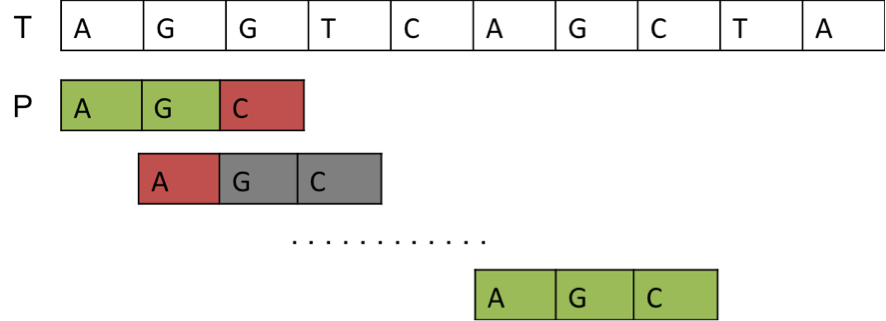
\includegraphics[scale=0.5]{Fuerza_Bruta.png}
		\rule{35em}{0.5pt}
	\caption[Ejemplo del algoritmo de fuerza bruta]{Ejemplo del algoritmo de fuerza bruta}
	\label{fig:FuerzaBruta}
\end{figure}
\end{example*}
\newcommand{\myrule} [3] []{
    \begin{center}
        \begin{tikzpicture}
            \draw[#2-#3, ultra thick, #1] (0,0) to (0.5\linewidth,0);
        \end{tikzpicture}
    \end{center}
}
\myrule{}{}
\subsection{Knuth Morris Pratt (KMP)}
\label{subsec:kmp}
El primer algoritmo que mejoró el orden de ejecución fue presentado por primera vez en junio de 1977 por Donald E. Knuth, James H. Morris y Vaughan R. Pratt \cite{KMP}.\\
A diferencia del algoritmo de fuerza bruta, KMP presenta la idea de saltar una secuencia de caracteres al ocurrir una diferencia ({\it missmatch}) entre un carácter del texto ({\it T}) y otro de {\it p} que se estén comparando.\\
Los autores de este algoritmo proponen realizar dos fases. En la primera se realiza la construcción de una tabla que indica cuántos caracteres se debe desplazar {\it p} con respecto al texto al ocurrir un fallo en la búsqueda. En la segunda fase se realiza una recorrida secuencial sobre el texto, comparando cada entrada con {\it p}. En caso de ocurrir un fallo se utiliza la tabla construida en la primera fase para conocer el desplazamiento que se debe realizar, en caso contrario se continua avanzando secuencialmente. Si se comparan con éxito los $m$ elementos de {\it p} con una sub secuencia del texto se tendrá una ocurrencia de {\it p} en el texto.
Este mecanismo permite evitar comparaciones que se sabe de ante mano serán inútiles, mejorando de esta forma el rendimiento de la búsqueda en comparación al algoritmo de fuerza bruta.\\
Para cada posición $i$, $i \leq \mid p \mid$, en el patrón {\it p}, definimos $sp_{i}'$ como el largo del sufijo más largo de $p[1..i]$ que es prefijo de {\it p} y además cumple que los caracteres $p[i+1]$ y $p[sp_{i}' + 1]$ son diferentes \cite{GUS}. 
\begin{example*}
Si consideramos $p = accgtacct$ se tiene que $sp_{1}' = sp_{2}' = sp_{3}' = sp_{4}' = sp_{5}' = 0$, $sp_{6}' = sp_{7} = 1$, $sp_{8}' = 3$.
\end{example*}
\myrule{}{}
Este algoritmo permite encontrar todas las ocurrencias de {\it p} en un {\it T} en $O(m+n)$.\\
Si consideramos $sp_{i}'$ como la función de fallos mencionada anteriormente, se puede definir el desplazamiento del algoritmo KMP en caso de fallos en términos de $sp_{i}'$. Dada una alineación de {\it p} y el texto, si ocurre un fallo en la comparación en la posición $i + 1$ respecto a {\it p} y $k$ respecto del texto, se debe desplazar el patrón $i - sp_{i}'$ posiciones hacia la derecha. De esta forma se tiene que $p[1,sp_{i}']$ se alinéa con $T[k-sp_{i}',k-1]$. Si una ocurrencia de {\it p} es encontrada en el texto se desplaza al patrón $m-sp_{m}'$ lugares.
\begin{example*}
Tomando $p = accgtacct$ y $T = accgtatttg$ se tiene que el algoritmo KMP al procesar el texto encuentra un fallo en la posición 7 ($i=6$). Como $sp_{6}' = 1$, el algoritmo KMP debe desplazar 5 posiciones a {\it p}. En la figura \ref{fig:matrix} se muestra la situación descrita.
\begin{center}
\begin{figure} [H]
\centering
$\begin{matrix}
0&   &   &   &   &   &   &   &   & 1\\
1& 2 & 3 & 4 & 5 & 6 & 7 & 8 & 9 & 0\\
a& c & c & g & t & a & t & t & t & g\\
a& c & c & g & t & a & c & c & t &  \\
 &   &   &   &   & a & c & c & g & t \\
\end{matrix}$
	\caption[Ejemplo del algoritmo KMP]{Ejemplo del algoritmo KMP}
	\label{fig:matrix}
\end{figure}
\end{center}
\end{example*}
\subsection{Boyer Moore (BM)}
Este algoritmo fue presentado por primera vez por Robert S Boyer y J Stother Moore en octubre de 1977 \cite{BM}. 
La versión original del algoritmo presenta mejoras prácticas a los algoritmos de búsqueda de cadenas de caracteres existentes hasta ese momento.\\
A diferencia de KMP, el algoritmo presentado en esta sub sección realiza las comparaciones entre caracteres de un patrón {\it p} y una porción de texto $T[i, \text{ } i \text{ } + \mid p \mid - \text{ } 1]$ de derecha a izquierda. El índice $i$, sin embargo avanza dentro de {\it T} de izquierda a derecha igual que en KMP.
Los autores introducen en su artículo dos funciones sobre las cuales se basa el algoritmo, estas funciones son $delta1$, conocida como regla del carácter malo ({\it bad character}) y $delta2$, conocida como regla del sufijo bueno ({\it good sufix}).
Estas dos funciones son obtenidas mediante la realización de un pre procesamiento sobre {\it p} y el alfabeto {\it A}.\\
El tiempo de ejecución en el peor caso de este algoritmo es $O(m + n)$.
\subsubsection{Regla del carácter malo}
Siguiendo el enfoque de \cite{GUS} definimos la función $R(x)$ para cada $x \in A$ como la posición más a la derecha del carácter $x$ en $p$, se asigna 0 a $R(x)$ si $x$ no se encuentra en $p$ .
Crear esta función implica una fase de pre procesamiento, en la cual se crea una tabla que contiene los valores de $R(x)$ para todos los símbolos del alfabeto.\\
Una vez realizado el pre procesamiento la función $R(x)$ es utilizada cuando ocurre un fallo al comparar una posición $i$ de $p$ con una posición $k$ del texto {\it T}. En este caso, la regla del carácter malo indica que {\it p} debe desplazarse $max\{1, \text{ } i - R(T[k])\}$ posiciones hacia la derecha.
\begin{example*}
En la figura \ref{fig:BadChar1} se presenta un fallo en $i=3$ y $k=4$. La regla del carácter malo indica que {\it p} debe desplazarse $max\{1, i - R(T[k])\}$ posiciones, es decir, $max\{1, \text{ } i - R(T[4])\}$ $=$ $max\{1, \text{ } 3 - 1\}$ $= 2$. Luego de este desplazamiento se tiene la configuración ilustrada en la figura \ref{fig:BadChar2}, siguiendo el razonamiento anterior {\it p} debe desplazarse nuevamente dos posiciones hacia la derecha. Luego de dicho desplazamiento se obtiene una ocurrencia de {\it p} sobre el texto. Esta última situación se presenta en la figura \ref{fig:BadChar3}.
\begin{figure}[H]
\centering
	\subfigure[Ocurre un fallo en $k=4$]{%
	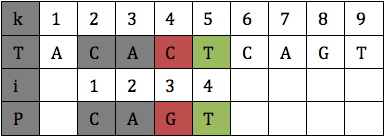
\includegraphics[scale=0.4]{BadCharStep1.png}
	\label{fig:BadChar1}}
\quad
	\subfigure[Ocurre un fallo en $k=7$]{%
	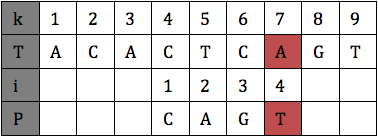
\includegraphics[scale=0.4]{BadCharStep2.png}
	\label{fig:BadChar2}}
\quad
	\subfigure[Se encuentra una ocurrencia de {\it p}]{%
	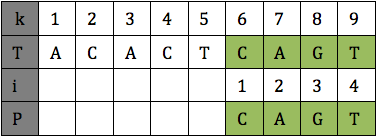
\includegraphics[scale=0.4]{BadCharStep3.png}
	\label{fig:BadChar3}}
\caption[Ejemplo de aplicación de la regla del carácter malo]{Ejemplo de aplicación de la regla del carácter malo}
\label{fig:BadChar}
\end{figure}
\end{example*}
\myrule{}{}
\subsubsection{Regla fuerte del sufijo bueno}
La regla del prefijo malo es útil cuando tenemos alfabetos extensos o se aplica en ambientes donde es altamente probable que ocurran fallos. Para los casos en que se tiene una probabilidad alta de fallo en posiciones finales de un patrón es útil la regla del sufijo bueno.\\
Supongamos que se comparan con éxito los últimos $t$ caracteres de {\it p} (de derecha a izquierda), pero el siguiente carácter falla. Sea $y$ el carácter de {\it p} en la posición $m – \mid t \mid - 1$ según {\it p} y el carácter $x$ de {\it T} alineado a $y$ tal que $x \not= y$.
En estas condiciones la \emph{regla del sufijo bueno} busca la secuencia $t’$ de {\it p} más a la derecha que cumpla que sea idéntica a $t$, que no sea sufijo de {\it p} y que además, $z$, el carácter inmediatamente a la izquierda de $t’$ sea distinto a $y$. Esta situación se ilustra en la figura \ref{fig:goodSufix1}.
\begin{figure}[H]
	\centering
		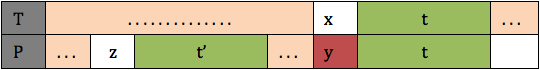
\includegraphics[scale=0.5]{GoodSufix1.png}
		\rule{35em}{0.5pt}
	\caption[Regla del sufijo bueno]{Regla del sufijo bueno}
	\label{fig:goodSufix1}
\end{figure}
Si no existe $t'$ pero existe $t''$ tal que $t''$ es sufijo de $t$ y existe una ocurrencia de $t''$ prefijo de $p$, se debe desplazar $p$ de forma tal que se logre la alineación entre $t''$ de $p$ y $t''$ de {\it T}. Este caso abarca el hecho de encontrar una ocurrencia de $p$ en el texto. En caso que $t''$ sea vacía, se debe desplazar $p$ $m$ posiciones hacia la derecha.\\
Formalizaremos los conceptos anteriormente explicados definiendo dos funciones $L'$ y $l'$.\\
Para cada índice $i=2..m$ de {\it p} se define $L'(i)$ como el máximo $j$, $j<m$, tal que $p[i,m]$ es sufijo de $p[1,j]$ y $p[i-1]$ no coincide con el carácter precedente del sufijo (es decir el carácter $p[j - \mid p[i,m] \mid]$).
Por último definimos $l’(i)$, $i > 1$, como la cantidad de caracteres del sufijo más largo de $p[i,n]$ que también es prefijo de {\it p}. De no existir dicho valor definimos  $l’(i)=0$.
\begin{example*}
Considerando $p=catgatgat$ tenemos que $L'(8)=3$ (Notar que $L'(8)\not=6$ porque $p[4]= p[i-1]=p[7]$), mientras que, para todo $1 \leq i \leq 10$, $l'(i)=0$.
\end{example*}
\myrule{}{}
Al procesar el texto se puede utilizar la regla del sufijo bueno cuando ocurre un fallo en la posición $i-1$ de $p$ de la siguiente forma:
\begin{itemize}
\item Si $L'(i) > 0$ se debe desplazar el patrón $p$ $(m - L'(i))$ posiciones hacia la derecha (esta situación es la presentada en la figura \ref{fig:goodSufix1}).
\item Si $L'(i) = 0$ ($t'$ es vacía) se debe deslpazar el patrón $p$ $(m - l'(i))$ posiciones hacia la derecha .
\end{itemize}
Si ocurre un fallo al comparar la posición {\it m-esíma} (primera comparación) se debe desplazar $p$ una posición a la derecha.
Al encontrar una ocurrencia del patrón $p$, se desplaza $p$ $(m - l(2)')$ posiciones hacia la derecha.
\section{Algoritmos de búsqueda exacta de múltiples patrones en un texto}
Dado un conjunto de patrones $P=\{p_{1}...p_{k}\}$, los algoritmos de búsqueda exacta de múltiples patrones en un texto hallan las ocurrencias de cada patrón de $P$ dentro de un texto.
Los algoritmos de este tipo que presentaremos en este documento se basan en las estructuras de datos {\it trie} y {\it árbol de sufijos} detalladas en las secciones \ref{sec:deftrie} y \ref{sec:defSufixTree} respectivamente.\\
Cabe notar que el algoritmo de Aho Corasick (capítulo \ref{Chapter2}) y MSW (capítulo \ref{Chapter3}) caen dentro de esta categoría, siendo el primero una solución clásica a este problema.
\subsection{Árbol de prefijos o Trie}
\label{sec:deftrie}
Definimos $\mathcal{T}$ como un \emph{trie} o árbol de prefijos de un conjunto de patrones {\emph P} sobre un alfabeto {\it A} si $\mathcal{T}$ es un árbol con raíz que cumple las siguientes propiedades \cite{GUS}:
\begin{itemize}
\item Cada arista de $\mathcal{T}$ se etiqueta con un único símbolo del alfabeto {\it A}.
\item Para todo par de aristas salientes de un nodo de $\mathcal{T}$ se cumple que sus etiquetas son diferentes.
\item Por cada patrón $p \in {\it P}$ existe un nodo {\it v} en $\mathcal{T}$ tal que la secuencia de caracteres resultantes de la concatenación de todos los símbolos en el camino desde el nodo raíz hasta el nodo {\it v} es igual a $p$.
\item La secuencia de caracteres que resulta de concatenar las etiquetas del camino desde el nodo raíz hasta cualquier hoja de $\mathcal{T}$ es un patrón que se encuentra en {\emph P}.
\end{itemize}
\begin{example*}
\label{ex:example1}
Sea \emph{P} un conjunto de patrones sobre un alfabeto \{a, c, g, t\} tal que \emph {P} = \{cg, acg, act, acta, cgg\}, la estructura {\it trie} resultante es la presentada en la figura \ref{fig:trie}. 
\begin{figure}[H]
\centering
\begin{tikzpicture}[every tree node/.style={draw,circle},fill=blue!20,
   level distance=1.75cm,sibling distance=0.8cm, 
   edge from parent path={(\tikzparentnode) -- (\tikzchildnode)}]
\Tree [.\node[fill=blue!20] {}; 
	\edge node[left] {a};  
    [.\node[fill=blue!20] {}; 
      \edge node[left] {c};  
      [.\node[fill=blue!20] {}; 
		   \edge node[left] {g};  
		   [.\node[fill=blue!20] {}; ] 
		   \edge node[right] {t};
	       [.\node[fill=blue!20] {}; 
	     	  \edge node[right] {a};
	     	  [.\node[fill=blue!20] {}; ] 
    		   ]
       ]
    ]
    	\edge node[right] {cg};  
    [.\node[fill=blue!20] {}; 
      \edge node[right] {g};
       [.\node[fill=blue!20] {}; ]
    ]
    ];
\end{tikzpicture}
\caption[Ejemplo: trie]{{\it trie}}
	\label{fig:trie}
\end{figure}
\end{example*}
\myrule{}{}
A continuación introducimos un conjunto de definiciones que aplican a un árbol $\mathcal{T}$ y alfabeto {\it A}, estas definiciones serán usadas a lo largo de todo este documento.
\begin{itemize}
\item Se define \emph{camino} en un árbol como cualquier secuencia de nodos $n_{1}...n_{k}$ que cumpla que cada nodo es padre del siguiente en la secuencia. La \emph{longitud} del camino se define como el número de arístas que se recorren, es decir el número de nodos de la secuencia menos uno ($k - 1$).
\item La \emph{profundidad de un nodo} se define como la longitud del camino que comienza en la raíz y termina en el nodo. La profundidad de la raíz es cero.
\item Asociamos a cada arista de $\mathcal{T}$ una secuencia de caracteres de {\it A} que llamaremos \emph{etiqueta} de la arista. En un trie, todas las aristas tienen etiquetas de largo 1.
\item Llamaremos \emph{etiqueta de un nodo} {\it v} (denotada $L(v)$) a la concatenación de las etiquetas de las aristas que se encuentran en el camino definido entre la raíz de $\mathcal{T}$ y {\it v}.
\item Si hay un camino del nodo {\it u} al nodo {\it v}, {\it u} es \emph{ascendiente} de {\it v} y {\it v} es \emph{descendiente} de {\it u}. Esta situación la notaremos como $v \prec u$
\end{itemize}
Esta estructura de datos sirve de base para el algoritmo de Aho Corasick (capítulo \ref{Chapter2}) y para resolver otro tipo de problemas de búsqueda en un texto. Por ejemplo, esta estructura puede ser utilizada para resolver el problema del diccionario ({\it dictionary problem}). En este problema un conjunto de patrones es insertado en un {\it Trie}, luego, se verifica si secuencias individuales de un texto pertenecen o no al diccionario (conjunto de patrones).
\subsection{Árbol de sufijos}
\label{sec:defSufixTree}
Un árbol de sufijos $\mathcal{T}$ para una secuencia de caracteres $s[1,m]$, en un alfabeto {\it A}, es un árbol con raíz que cumple las siguientes propiedades \cite{GUS}:
\begin{itemize}
\item El árbol tiene exactamente $m$ hojas.
\item Cada nodo interno tiene al menos dos nodos descendientes, salvo, potencialmente, el nodo raíz.
\item Cada arista se etiqueta con una cadena de caracteres no vacía.
\item Dado un nodo $v$ del árbol, no existen dos aristas salientes de $v$ que coincidan en el primer carácter de sus etiquetas.
\item Cada hoja $v$ de $\mathcal{T}$ cumple que $L(v)$ es un sufijo de $s$.
\end{itemize}
\begin{example*}
En la figura \ref{fig:sufixTree1} se presenta un árbol de sufijos construido a partir de $s=tactag$
\begin{figure}[H]
\centering
\begin{tikzpicture}[every tree node/.style={draw,circle},fill=blue!20,
   level distance=1.75cm,sibling distance=0.8cm, 
   edge from parent path={(\tikzparentnode) -- (\tikzchildnode)}]
\Tree [.\node[fill=blue!20] {}; 
	\edge node[left] {a};  
    [.\node[fill=blue!20] {}; 
      \edge node[left] {ctag};  
      [.\node[fill=blue!20] {};  ]
      \edge node[right] {g};
       [.\node[fill=blue!20] {}; ]
    ]
    \edge node[left] {ctag};
    [.\node[fill=blue!20] {};]
    \edge node[right] {g};
    [.\node[fill=blue!20] {};]
    	\edge node[right] {ta};  
    [.\node[fill=blue!20] {}; 
      \edge node[left] {ctag};  
      [.\node[fill=blue!20] {};  ]
      \edge node[right] {g};
       [.\node[fill=blue!20] {}; ]
    ]
    ];
\end{tikzpicture}
\caption[Ejemplo: Árbol de sufijos]{Árbol de sufijos construído a partir de $s=tactag$}
	\label{fig:sufixTree1}
\end{figure}
\end{example*}
\myrule{}{}
Estos árboles pueden ser representados de forma compacta, etiquetando las aristas con el índice inicial y final. Esto es, cada arista etiquetada con una sub secuencia $s[i,j]$ es representada mediante los índices $i$ y $j$. Por ejemplo, tomando $s=tactag$, la arista etiquetada por $ctag$ queda representada por $(3,6)$.\\
Si un sufijo $w$ de $s$ es prefijo de otro sufijo $s$ no se podrá construir un árbol de sufijos a partir de $s$ ya que el nodo correspondiente a $L(w)$ no será una hoja. Por ejemplo, si consideramos $s=tagcag$, no se puede construir un árbol de sufijos con la definición anteriormente dada ya que el sufijo $w=ag$ es prefijo del también sufijo $agcag$. Para evitar este problema podemos agregar al final de $s$ un carácter especial $\$$ no perteneciente a {\it A}.\\
El algoritmo de Ukkonen \cite{UK95} o el algoritmo de Weiner \cite{WEINER} permiten construir un árbol de sufijos partiendo de una secuencia de caracteres $s$, $\mid s \mid =n$, en tiempo $O(n)$.\\
Esta estructura de datos nos permite buscar un patrón $p$, $\mid p \mid = m$, dentro de un texto en un tiempo $O(n+m)$. Para ello se construye el árbol de sufijos de texto {\it T} y luego se comparan los caracteres de $p$ comenzando del nodo raíz y descendiendo por las aristas del árbol que coincidan con $p$. Si es posible encontrar una coincidencia completa de $p$ existirán $z$ hojas debajo del camino recorrido, cada una de ellas es el comienzo de una ocurrencia de $p$. Si no es posible encontrar una coincidencia completa de $p$ en el árbol no se habrá encontrado ninguna ocurrencia del patrón en el texto.\\
El árbol de sufijos se puede generalizar de forma tal que se inserten sobre un mismo árbol de sufijos un conjunto de múltiples secuencias de caracteres $S=\{s_{1}..s_{k}\}$.\\
La estrategia de construcción más simple de este árbol de sufijos generalizado es concatenar todas las secuencias de forma tal que se defina una nueva secuencia $c=s_{1}\$_{1}..s_{k}\$_{k}$ donde $\$_{i}$ no pertenece al alfabeto y representa una marca única que identifica la finalización de una secuencia $s_{i}$. Luego se crea un árbol de sufijos partiendo de $c$, etiquetando a cada hoja con una tupla $(i,j)$, donde $i$ identifica la secuencia y $j$ el índice de comienzo de la secuencia $s_{i}$.\\
Otra forma de construir este árbol es agregar una a una las secuencias de $S$, utilizando de forma incremental el algoritmo de Ukkonen.

% Chapter 2

\chapter{Aho Corasick} % Main chapter title

\label{Chapter2}

\lhead{Capítulo 3. \emph{Aho Corasick}}

En este capítulo presentamos el algoritmo conocido con el nombre de Aho Corasick (AC) \cite{AC75}. Dicho algoritmo permite encontrar ocurrencias de múltiples patrones en un texto, basándose para ello en el uso de tres funciones que pueden ser representadas mediante la construcción de un grafo. Una vez generada esta estructura de datos la misma puede utilizarse para buscar los patrones sobre un texto en una sola recorrida.\\
Construir esta estructura demanda un tiempo de orden lineal en la suma de los largos de los patrones. Por otro lado, el tiempo que AC tarda en realizar el procesamiento del texto es de orden lineal en el largo del mismo más la cantidad total de ocurrencias de los patrones en el texto {\footnote{Observar que, si hay patrones prefijos de otros, pueden ocurrir múltiples reconocimientos de patrones en cada posición del texto}}.\\ Consideremos P, un conjunto de k patrones, cuya suma de largos (es decir la sumatoria de los largos de cada patrón perteneciente a P) es $m$, {\it T} el {\emph texto} con largo $n$ y h la cantidad de apariciones de los patrones de P en T. En estas condiciones, el tiempo de ejecución del algoritmo AC es de orden $n + m + h$. \\

\section{Algoritmo}
\label{sec:algoritmo_AC}
El algoritmo AC se basa en la construcción de una estructura de datos que puede utilizarse como una máquina de estados finita. Cada nodo dentro de esta estructura puede considerarse un estado en la etapa de procesamiento del texto, a su vez, en cada estado el algoritmo AC puede reconocer varios patrones.\\
Para construir esta máquina de estados, todos los patrones a ser buscados en el texto son insertados en un trie (definido en la sección \ref{sec:deftrie}). Sobre este trie, cuyos nodos serán los estados de la máquina, se representan tres funciones que definen el comportamiento del algoritmo AC. 
\begin{itemize}
\item Función de movimiento ({\it goto}) - Dado un estado {\it v} del trie y un símbolo {\it a} del alfabeto, retorna un estado {\it w} que es descendiente de {\it v} y la arista que los une está etiquetada con {\it a}. Si tal símbolo no existe, retorna vacío (salvo cuando $v$ es la raíz, en cuyo caso se retorna $v$).
\item Función de fallos ({\it failure}) - Dado un estado {\it v}, esta función retorna el estado de mayor profundidad existente en la estructura, $w$, tal que $L(w)$ es sufijo de $L(v)$, donde recordamos que $L(.)$ denota la etiqueta de un nodo, definida en la sección \ref{sec:deftrie}.
\item Función de salida ({\it output}) - Retorna el conjunto de patrones reconocidos en un estado determinado.
\end{itemize}
Cabe destacar que esta función de fallos es una generalización directa de la función de fallos definida en el algoritmo de KMP (sub sección \ref{subsec:kmp} del capítulo \ref{Chapter1}).\\
Estas funciones son construidas en dos etapas, en la primera se define la función {\it goto} y se crea una primera aproximación de la función {\it output}, mientras en la segunda se construye {\it failure} y se finaliza la creación de {\it output}. Las aristas del \emph{trie} definen, para todos los nodos distintos de la raíz, a la función {\it goto}. Cada nodo del trie representa un carácter de uno o más patrones (un nodo puede ser compartido por varios patrones). Por motivos de implementación (está contemplado en \cite{AC75}) en el estado raíz, la función {\it goto} debe ser completa, es decir, para todos los símbolos del alfabeto debe retornar un estado. Dependiendo del juego de patrones, es posible que para algún símbolo no existan descendientes del nodo raíz, para estos casos la función {\it goto} retorna el nodo raíz. En los nodos que no son raíz la función {\it goto} evaluada para un símbolo {\it a} del alfabeto retorna vacío si no existe un nodo descendiente en la dirección de {\it a}. La definición de {\it goto} puede resumirse de la siguiente forma.
\begin{itemize}
\item {\it goto(v,a) = w} - Si una arista {\it (v,w)} está etiquetada por un símbolo {\it a}.
\item {\it goto(0,a) = 0} - Si no existe una arista {\it (0,w)} etiquetada por el símbolo {\it a}, siendo 0 el nodo raíz del trie (utilizaremos esta notación a lo largo del capítulo).
\item {\it goto(v,a) = $\emptyset$} - En otros casos  (siendo {\it v} un nodo diferente de 0 y {\it a} un símbolo del alfabeto).
\end{itemize}
\begin{example*}
En la figura \ref{fig:goto_function} se presenta la función {\it goto} sobre el \emph{trie} del ejemplo \ref{ex:example1} presentado en el capítulo \ref{Chapter1}. Como puede observarse sólo se añade sobre el \emph{trie} un ciclo en el nodo raíz, de forma que, para todo símbolo x se tenga {\it goto(0,x)$\not= \emptyset$}. Todas las aristas del nuevo \emph{trie} representan la función {\it goto}.
\begin{figure}[H]
\centering
\begin{tikzpicture} [->,>=stealth',scale=.8,auto,node distance=2.0cm]
  \tikzstyle{every state}=[fill=blue!20,draw=none,text=white]

  \node[state]		   (A)                    {0};
  \node[state]         (B) [below left of=A] {A};
  \node[state]         (C) [below right of=A] {B};
  \node[state]         (D) [below of=B] {C};
  \node[state]         (F) [below of=D] {E};
  \node[state]         (E) [below of=C] {D};
  \node[state]         (G) [below left of=E] {F};
  \node[state]         (H) [below right of=E] {G};
  \node[state]         (I) [below of=H] {H};

  \path (A) edge              node {c} (B)
            edge              node {a} (C)
            edge [color=red, loop above] node {g,t} (A)
        (B) edge 			 node {g} (D)
        (D) edge              node {g} (F)
        (C) edge              node {c} (E)
        (E) edge              node {g} (G)
        		edge              node {t} (H)
		(H) edge              node {a} (I);
\end{tikzpicture}
\caption[Ejemplo: Función goto]{Función {\it goto}}
	\label{fig:goto_function}
\end{figure}
\end{example*}
\myrule{}{}
La primera fase de construcción de {\it output} se realiza al construir la función {\it goto}. En esta etapa se le asigna a los nodos cuya etiqueta coincide con un patrón, un valor que indica que dicho nodo representa el final de un patrón. 
En la segunda etapa se procede a construir {\it failure} y finalizar la construcción de {\it output}, mediante el algoritmo de Aho  Corasick \cite{AC75} que presentamos en el algoritmo {\ref{Algorithm:failure_step2}.
En la primera línea del algoritmo se inicializa una variable {\it queue}, que se utiliza para realizar una recorrida BFS sobre el \emph{trie}, creando así a la función {\it failure} por niveles de profundidad. La creación de {\it failure} consta de dos pasos. El primer paso se realiza en el ciclo presentado entre las líneas 2 y 6. En este se inicializa la función {\it failure} para todos los nodos del \emph{trie} con profundidad 1, de forma tal que la función {\it failure} sobre estos nodos retorne el nodo raíz ({\it failure(s) = 0}). Estos nodos son insertados en la cola {\it queue} y, de aquí en más, sólo se agregarán nodos a {\it queue} para los cuales $failure$ ya haya sido definida.
\begin{algorithm}[h]
\small
\caption{Creación de la función {\it failure} y segunda fase de creación de {\it output} }
\label{Algorithm:failure_step2}
\begin{algorithmic}[1]
\State $queue \gets empty$
\ForAll {a such that {\it goto(0,a)$\not= 0$}}
	\State $s \gets goto(0,a)$
	\State $failure(s) \gets 0$
	\State $queue \gets queue \cup \{s\}$	
\EndFor
\While {queue $\not= empty$ }
	\State $r \gets getNext(queue)$	
	\State $queue \gets queue - \{r\}$
	\ForAll {a such that {\it goto(r,a) $\not= \emptyset$}}
		\State $s \gets goto(r,a)$
		\State $state \gets {\it failure(r)}$	
		\While {{\it goto(state, a) = $\emptyset$}}
			\State $state \gets {\it failure(state)}$
		\EndWhile
		\State ${\it failure(s)} \gets {\it goto(state,a)}$
		\State ${\it output(s)} \gets {\it output(s)} \cup {\it output({\it failure(s)})}$
		\State $queue \gets queue \cup \{s\}$	
	\EndFor
\EndWhile
\Statex
\end{algorithmic}
  \vspace{-0.4cm}%
\end{algorithm}
La segunda etapa del algoritmo de creación de {\it failure} se realiza en el segundo ciclo (líneas 7 a 20). Este ciclo hace una recorrida BFS sobre todos los nodos del \emph{trie}, comenzando con los nodos de profundidad 1. Llamamos {\it r} al nodo que se retira de la cola {\it queue} en cada iteración. En el ciclo de la línea 10, la variable $s$ itera sobre todos los descendientes de {\it r} con etiqueta ${\it a} \in {\it A}$. En la línea 12 definimos {\it state} como el resultado de la función {\it failure(r)} (notar que $failure$ ya fue definido para $r$ porque $r$ fue sacado de la cola). El ciclo comprendido entre las líneas 13 y 15 itera aplicando la función $failure$ a $state$ sucesivamente, hasta que se alcanza un nodo tal que goto(state, a)$\not= \emptyset$. Cabe señalar que este ciclo siempre finaliza ya que {\it goto(0, a)$\not= \emptyset$ } y además la función $failure(r)$ retorna siempre un nodo de menor profundidad que $r$. La función {\it failure(s)} queda definida en la línea 16.\\
Por otro lado, en la línea 17 se completa la construcción de la función {\it output(s)} mediante la unión de todos los patrones reconocidos en s ({\it output(s)}) y todos los patrones que sean sufijos de {\it s} ({\it output(failure(s))}). El resultado final de este algoritmo es una estructura de datos que contiene las tres funciones necesarias para buscar ocurrencias de patrones sobre un texto.
\begin{example*}
Agregando la función de fallos al ejemplo de la figura \ref{fig:goto_function}, representada por las aristas punteadas, se tiene que la estructura final queda como se muestra en la figura  \ref{fig:failure_function}. Consideremos el nodo F de la figura \ref{fig:failure_function}, la función de salida de este nodo debe contener tanto el patrón acg como cg, ya que el último es un sufijo del primero y ambos pertenecen al juego de patrones que se desea hallar.
\begin{figure}[H]
\centering
\begin{tikzpicture} [->,>=stealth',scale=.8,auto,node distance=2.0cm]
  \tikzstyle{every state}=[fill=blue!20,draw=none,text=white]

  \node[state]		   (A)                    {0};
  \node[state]         (B) [below left of=A] {A};
  \node[state]         (C) [below right of=A] {B};
  \node[state]         (D) [below of=B] {C};
  \node[state]         (F) [below of=D] {E};
  \node[state]         (E) [below of=C] {D};
  \node[state]         (G) [below left of=E] {F};
  \node[state]         (H) [below right of=E] {G};
  \node[state]         (I) [below of=H] {H};

  \path
  		(A) edge              node {c} (B)
            edge              node {a} (C)
            edge [loop above] node {g,t} (A)
        (B) edge 			 node {g} (D)
        (D) edge              node {g} (F)
        (C) edge              node {c} (E)
        (E) edge              node {g} (G)
        		edge              node {t} (H)
		(H) edge              node {a} (I);
	\path 
		(B) edge	 [dashed, bend left=20] node {} (A)
		(C) edge	 [dashed, bend right=30] node {} (A)
		(D) edge	 [dashed, bend left=70] node {} (A)
		(F) edge	 [dashed, bend left=60] node {} (A)
		(E) edge	 [dashed, bend right=40] node {} (B)
		(G) edge	 [dashed, bend left=20] node {} (D)
		(H) edge	 [dashed, bend right=50] node {} (A)
		(I) edge	 [dashed, bend right=40] node {} (C);
\end{tikzpicture}
\caption[Ejemplo: función goto y failure]{Función goto y failure}
	\label{fig:failure_function}
\end{figure}
\end{example*}
\myrule{}{}
Una vez construida la estructura de datos descrita en esta sección, se utiliza la misma como se muestra en el algoritmo {\ref{Algorithm:failure_step1}}.\\
\begin{algorithm}[h]
\small
\caption{Utilización de la estructura AC para reconocer patrones en un {\emph texto}}
\label{Algorithm:failure_step1}
\begin{algorithmic}[1]
	\State $st \gets 0$
	\ForAll {$i = 1..n$}
		\While {{\it goto(st, $T[i]$) = $\emptyset$}}
			\State $st \gets {\it failure(st)}$
		\EndWhile	
		\If {\it output(st) $\not= \emptyset$}
			\State Incrementar el contador de ocurrencias de todos los elementos de output(st).
		\EndIf
	\EndFor
	\Statex
\end{algorithmic}
  \vspace{-0.4cm}%
\end{algorithm}
Comenzando en el nodo 0 de la estructura se procede a leer secuencialmente cada uno de los caracteres del {\emph texto}. Dado un estado {\it st}, al leer un carácter $T[i]$ del {\emph texto}, se invoca en primera instancia la función {\it goto(st,$T[i]$)}, si dicha función falla se realiza una nevegación hacia {\it st = failure(st)} y se repite el procedimiento con el nuevo nodo {\it st}. Si por el contrario {\it goto(st,$T[i]) \not= \emptyset$}, se realiza una navegación hacia {\it st} y se invoca {\it output(st)}. En caso que la función {\it output(st)} no sea vacía se habrá encontrado al menos un acierto.
\section{Implementación}
En esta sección se describen los aspectos más relevantes de la implementación en lenguaje C++ del algoritmo AC realizada para este proyecto. \\
Como se explicó en la sección anterior, la construcción de la estructura de datos de AC se realiza en etapas. En la etapa más temprana (cuando se agregan los patrones) la estructura coincide con una estructura trie. No es necesario almacenar de forma explícita los caracteres que forman cada uno de los patrones, ya que dicha información queda representada implícitamente en la relación nodo padre - nodo hijo. En fases posteriores de la construcción de la estructura de AC, se realiza (sobre el trie) una secuencia de pasos para construir las funciones {\it goto}, {\it failure} y {\it output}.\\
La estructura arborescente se conserva luego de construir dichas funciones, pero sobre los nodos del árbol se agregan aristas y vectores que definen a {\it failure} y {\it output} respectivamente. Considerando la estructura completa (con las aristas del árbol original y las añadidas para definir {\it failure}) se tiene una estructura final de grafo.\\
La definición de la estructura de AC se encuentra en {\bf AhoCorasickNode.h}, la misma tiene cuatro atributos sobre los cuales se basa (Ver el fragmento de código {\ref{lst:codigo_1}}).
\lstset { %
    language=C++,
    backgroundcolor=\color{black!5}, % set backgroundcolor
    basicstyle=\footnotesize,% basic font setting
}
\begin{lstlisting}[caption=Representación de los nodos en AC, label={lst:codigo_1}]
AhoCorasickNode *children [ALPHABET_SIZE];
AhoCorasickNode *fail;
int *output;
int outputcount;
\end{lstlisting}
La constante {\bf ALPHABET\_SIZE} representa la cantidad de caracteres del alfabeto (por más información ver el apéndice \ref{AppendixB}).El arreglo  {\it children} representa la función {\it goto} en cada nodo.\\
El puntero {\it fail} define para cada nodo la función {\it failure}. \\
La función {\it output} es representada mediante un arreglo dinámico de enteros y un contador ({\it outputcount}) que almacena la cantidad de datos presentes en dicho vector. A cada uno de los patrones insertados en la estructura se le asigna un identificador secuencial numérico; estos valores son guardados (cuando corresponde hacerlo) dentro de {\it output}. Otra posible implementación de {\it output} se obtiene al usar la clase {\it Vector} de la {\it standard template library}, sin embargo, nuestras pruebas mostraron que una implementación así resulta más costosa en tiempo de ejecución. \\
Cada patrón es insertado en AC invocando al método {\it addPattern}, el cual se encuentra implementado en el módulo {\bf AhoCorasickGraph}. Este método recibe como parámetro una cadena de caracteres (la cual representa a un patrón) y el identificador que se le asignó a dicho patrón. Como puede apreciarse en el fragmento de código {\ref{lst:codigo_2}}, este procedimiento comienza la inserción partiendo desde el nodo raíz del árbol AC, luego, para cada carácter del patrón {\it word} el procedimiento analiza si ya existe o no un nodo en la estructura que represente a la secuencia leída hasta el momento. Se utiliza un arreglo, al cual nombramos \emph{ordchar}, para obtener en O(1) el índice que tiene asignado cada símbolo del alfabeto (representado en ASCII) en el arreglo de descendientes ({\it children}). Finalmente {\it addPattern} realiza un movimiento en la estructura en dirección al carácter procesado; en caso de que no exista un nodo en dicha dirección el mismo es creado.

\begin{lstlisting}[caption=Representación de los nodos en AC, label={lst:codigo_2}]
void AhoCorasickGraph::addPattern(const char* word,
 int wordIndex) {
	AhoCorasickNode* currentNode = root;
	AhoCorasickNode* child = NULL;
	int index = 0;
	int aux;
	while (word[index] != '\0') {
        aux = ordChar[(int) word[index]];
		child = currentNode->children[aux];
		if (!child) {
			child = new AhoCorasickNode();
			currentNode->children[aux] = child;
		}
		currentNode = child;
		index++;
	}
	currentNode->addOutput(wordIndex);
}
\end{lstlisting}

Una vez se insertan todos los patrones a la estructura inicial se procede con la ejecución del método {\it setFailTransitions}. Este método completa la función {\it goto} en el nodo raíz e implementa las dos fases descritas en el algoritmo {\ref{Algorithm:failure_step2}}.
La implementación de este método se muestra en el fragmento de código {\ref{lst:codigo_3}}
\begin{lstlisting}[caption=Creación de la función failure, label={lst:codigo_3}]
void AhoCorasickGraph::setFailTransitions(int numberOfPatterns) {
    founds = (int*)calloc(numberOfPatterns, sizeof(int));
	Queue* queue = new Queue();
	//1) f(s) <- 0 para todo s con profundidad 1
	AhoCorasickNode* child = NULL;
	AhoCorasickNode* state = NULL;
	int currentSymbol;
	for (int childIndex = 0; childIndex < ALPHABET_SIZE;
	 childIndex++) {
		currentSymbol = (int) ordChar[(int)alphabet[childIndex]];
		child = root->children[currentSymbol];
		if (child) {
			child->fail = root;
			queue->addNode(child);
		}
		else {
			root->children[currentSymbol] = root;
		}
	}
	//2) se configura failure en los estados con profundidad d > 1
	while (!queue->isEmpty()) {
		AhoCorasickNode* r = queue->getNextNode();
		for (int childIndex = 0; childIndex < ALPHABET_SIZE;
		 childIndex++) {
			currentSymbol = ordChar[(int)alphabet[childIndex]];
			child = r->children[currentSymbol];
			if (child) {
				queue->addNode(child);
				state = r->fail;
				while (!state->children[currentSymbol]) {
					state = state->fail;
				}
				child->fail = state->children[currentSymbol];
				child->outputUnion();
			}
		}
	}
	delete queue;
}
\end{lstlisting}
El procedimiento {\it setFailTransitions} también crea una tabla ({\it founds}) que es utilizada para almacenar la cantidad de apariciones de cada patrón en el texto. Otra posible solución al problema de almacenar la cantidad de ocurrencias de cada patrón en el texto es agregar a la definición del nodo AC un atributo que cuente las veces que el algoritmo de procesamiento pasa por cada nodo. La desventaja de hacer la implementación de esa forma es que todos los nodos que no representen el reconocimiento de algún patrón deben almacenar un entero que no se modificará. Además, como un mismo patrón puede ser reconocido en varios nodos (en el ejemplo de la figura \ref{fig:failure_function} el patrón "cg" es reconocido en los nodos C y F) sería necesario implementar una etapa de post procesamiento para obtener la cantidad de veces que se encuentra cada uno de los patrones dentro del {\emph texto} procesado.\\
El procedimiento {\it outputUnion} implementa la unión de patrones a ser reconocidos en el nodo que lo invoca, la definición de esta función se presenta en la línea 16 del algoritmo {\ref{Algorithm:failure_step2}}.\\
Una vez finalizada la construcción de la estructura de datos se procesa el texto. Cada bloque leído del  texto es enviado al procedimiento {\it updateGraph}. Este procedimiento actualiza la posición actual dentro de la estructura de datos y la tabla {\it founds} a partir de cada carácter del bloque.\\
El código {\ref{lst:codigo_4}} es una implementación del algoritmo \ref{Algorithm:failure_step1}.
\begin{lstlisting}[caption=Actualización de la estructura , label={lst:codigo_4}]
void AhoCorasickGraph::updateGraph(char block[], size_t bytCount) {
    int alphabetIndex;
    for (Uint blockIndex = 0; blockIndex < bytCount; blockIndex++) {
        alphabetIndex = ordChar[(int)block[blockIndex]];
        AhoCorasickNode* nextNode = currentPosition->children[alphabetIndex];
        while (!nextNode) {
            nextNode = currentPosition->fail;
            currentPosition = nextNode;
            nextNode = currentPosition->children[alphabetIndex];
        }
        currentPosition = nextNode;
        int oLength = currentPosition->outputcount;
        for (int outputIndex = 0; outputIndex < oLength; outputIndex++) {
            founds[currentPosition->output[outputIndex]] += 1;
        }
    }
}
\end{lstlisting}
La destrucción de la estructura se realiza en forma recursiva, recorriendo las aristas que forman el árbol en profunidad. Al momento de realizar la destrucción de la estructura se debe recordar que en el nodo ráiz se pueden presentar ciclos (causados por la función {\it goto}), por este motivo se identifica este nodo mediante la asignación de {\it outputcount} en -1. 
% Chapter 1

\chapter{Algoritmo basado en la clausura FSM de un árbol de patrones (MSW)} % Main chapter title

\label{Chapter3} % For referencing the chapter elsewhere, use \ref{Chapter3} 

\lhead{Chapter 4. \emph{Algoritmo basado en la clausura FSM de un árbol de patrones (MSW)}}
En este capítulo se presenta el algoritmo MSW (sección \ref{sec:algoritmo_MSW}) y una implementación del mismo en C++ (sección \ref{sec:Implementacion}). El algoritmo MSW permite realizar la búsqueda de múltiples patrones sobre un texto, basándose para ello en la construcción de una máquina de estados (\textbf{FSM}) que es creada a partir de una estructura arborescente (la cual representa todos los patrones) definida en la sub sección \ref{subsec:gct}. Resulta necesario introducir un conjunto de definiciones para presentar el algoritmo MSW, estas definiciones se encuentran en la sección \ref{section:def_prev}.
%Definiciones previas?
\section{Definiciones previas}
\label{section:def_prev}
En esta sección se presenta un conjunto de definiciones que serán utilizadas para describir el algoritmo MSW.
En esta sección se presenta un conjunto de definiciones que serán utilizadas para describir el algoritmo MSW.
\subsection{Árbol GCT}
\label{subsec:gct}
Diremos que un árbol $\mathcal{T}$, con raíz,  es un {\it General Context Tree} (\textbf{GCT}) si cumple las siguientes propiedades \cite{MSW04}:
\begin{itemize}
\item Cada arista está etiquetada por una secuencia de símbolos pertenecientes a {\it $A^{+}$}, siendo {\it $A^{+}$} el conjunto de secuencias de símbolos del alfabeto {\it A} de largo positivo.
\item Cada nodo puede tener hasta $\mid A \mid$ aristas salientes.
\item Cada nodo es etiquetado mediante una secuencia finita de caracteres resultante de concatenar las etiquetas de las aristas del camino que une a la raíz con el nodo. El nodo raíz es etiquetado con 0. Identificamos los nodos con sus etiquetas y así decimos, por ejemplo, que un nodo es prefijo de otro para indicar que sus etiquetas satisfacen esa condición.
\end{itemize}
La estructura GCT, o estructuras que comparten propiedades similares también se conocen con el nombre de árbol PATRICIA \cite{PAT}. Cabe observar que un {\it Trie} (definido en el capítulo \ref{Chapter2}) es un caso particular de GCT, donde todas las etiquetas de las aristas son de largo 1.
\begin{example*}
En la figura \ref{fig:gct} se presenta un árbol GCT construido sobre el alfabeto \{a, c, g, t \}.
\begin{figure}[H]
\centering
\begin{tikzpicture}[every tree node/.style={draw,circle},fill=blue!20,
   level distance=1.75cm,sibling distance=0.8cm, 
   edge from parent path={(\tikzparentnode) -- (\tikzchildnode)}]
\Tree [.\node[fill=blue!20] {}; 
	\edge node[left] {ag};  
    [.\node[fill=blue!20] {}; 
      \edge node[left] {gt};  
      [.\node[fill=blue!20] {};  ]
      \edge node[right] {c};
       [.\node[fill=blue!20] {}; ]
    ]
    \edge node[left] {gc};
    [.\node[fill=blue!20] {};]
    \edge node[right] {ccc};
    [.\node[fill=blue!20] {};]
    ];
\end{tikzpicture}
\caption[Ejemplo: GCT]{GCT construido sobre el alfabeto \{a, c, g, t \}}
	\label{fig:gct}
\end{figure}
\end{example*}
\myrule{}{}
\subsection{Descomposición canónica}
\label{subsec:desc_canonica}
En esta subsección definimos la \emph{descomposición canónica}, su implementación y uso dentro del algoritmo MSW serán abordados en el capítulo \ref{sec:algoritmo_MSW}.\\
Diremos que una secuencia {\it w} es una \emph{palabra} de $\mathcal{T}$ si es prefijo de un nodo de $\mathcal{T}$.\\
%Diremos que un estado {\it s} $\in$ {\it T} ({\it T} un árbol GCT) es un {\bf estado permanente} de {\it T} si y solo si $deg(s) < \alpha$ \footnote{{\it deg(s)} representa el número de aristas salientes del estado {\it s}} o {\it s} tiene una arista compuesta.
Dada una secuencia de caracteres {\it y} $\in$ {\it $A^{*}$}, donde {\it $A^{*}$} es el conjunto finito de secuencias de símbolos del alfabeto {\it A}, definimos la descomposición canónica {\it $C_{\mathcal{T}}$(y)} =  $\langle$ r, u, v $\rangle$, r, u, v $\in$ {\it $A^{*}$}, donde  $y = ruv$, $r$ es el prefijo más largo de {\it y} que es nodo de $\mathcal{T}$ y $ru$ es el prefijo más largo de {\it y} que es palabra de $\mathcal{T}$. 
\begin{example*}
Tomando como $\mathcal{T}$ el árbol de la figura \ref{fig:gct}, tenemos que {\it $C_{\mathcal{T}}$(aggc)} = $\langle$ ag, g, c $\rangle$.\\
\end{example*}
\myrule{}{}
\subsection{Árbol $\mathcal{T}_{suf}$}
Dado un GCT, $\mathcal{T}$, definimos $\mathcal{T}_{suf}$ como el GCT que se obtiene a partir de $\mathcal{T}$ agregando como nodos todos los sufijos de los nodos.
\begin{example*}
Partiendo del árbol de la figura \ref{fig:gct}, se construye el árbol $\mathcal{T}_{suf}$ presentado en la figura \ref{fig:tsuf}.
\begin{figure}[H]
\centering
\begin{tikzpicture}[every tree node/.style={draw,circle},fill=blue!20,
   level distance=1.75cm,sibling distance=0.8cm, 
   edge from parent path={(\tikzparentnode) -- (\tikzchildnode)}]
\Tree [.\node[fill=blue!20] {}; 
	\edge node[left] {ag};  
    [.\node[fill=blue!20] {}; 
      \edge node[left] {gt};  
      [.\node[fill=blue!20] {};  ]
      \edge node[right] {c};
       [.\node[fill=blue!20] {}; ]
    ]
    \edge node[right] {g};
    [.\node[fill=blue!20] {};
	  \edge node[left] {t};
      [.\node[fill=blue!20] {};] 
      \edge node[right] {c};
      [.\node[fill=blue!20] {}; ]
      \edge node[right] {gt};
       [.\node[fill=blue!20] {}; ]
    ] 
    \edge node[right] {c};
    [.\node[fill=blue!20] {};
	  \edge node[right] {c};
      [.\node[fill=blue!20] {};
		\edge node[right] {c};
      	[.\node[fill=blue!20] {};]
      ]
    ]
	\edge node[right] {t};
    [.\node[fill=blue!20] {};
	]    
    ];
\end{tikzpicture}
\caption[Ejemplo: $\mathcal{T}_{suf}$]{$\mathcal{T}_{suf}$ construido a partir del árbol de la figura \ref{fig:gct}}
	\label{fig:tsuf}
\end{figure}
\end{example*}
\myrule{}{}
\subsection{Clausura FSM sobre un árbol $\mathcal{T}$}
\label{subsec:clausura_FSM}
%comienza guia de Alvaro
Los GCT se usan en \cite{MSW04} como un mecanismo de selección de estados para asignar una probabilidad al siguiente carácter de un texto condicionado en los anteriores, de forma similar al uso de máquinas de estado finitas en modelos Markovianos. Específicamente, el \emph{estado} seleccionado por $T[1,i]$ en un GCT $\mathcal{T}$ es el nodo $r$ de la descomposición canónica $C_{\mathcal{T}}$(y)} =  $\langle$ r, u, v $\rangle$, donde $y=T[i]T[i-1]...T[1]$ es el reverso de $T[1,i]$.\\
El algoritmo de búsqueda de patrones que presentamos en este capítulo construye un GCT a partir de un conjunto de patrones $P=\{p_{1}..p_{k}\}$ y utiliza este mecanismo de selección de estados para identificar ocurrencias de patrones en el texto. Concretamente, a partir de un GCT que contiene sólo la raíz se construye $\mathcal{T}$ agregando, de forma secuencial, los nodos correspondientes a $\overline{p_{1}}, \overline{p_{2}}, ..., \overline{p_{k}}$, donde $\overline{p_{j}}$ es el reverso de $p_{j}$. La inserción de $\overline{p_{j}}$ en $\mathcal{T}$ con descomposición canónica $C_{\mathcal{T}}(\overline{p_{j}}) = \langle r, u, v \rangle$ implica la creación de un nodo $ruv$ y la potencial creación de un nodo $ru$ si $v \not= 0$. En este último caso, el estado $ru$ no representa ningún patrón de P, sino que se crea para satisfacer requerimientos estructurales de los GCT. En este GCT, cada vez que un patrón $p_{j}$ ocurre en el texto, digamos como sufijo de $T[1,i]$, para algún $i$, $\mid p_{j} \mid \leq i \leq \mid T \mid$, el estado seleccionado por $T[1,i]$ será el que representa a $\overline{p_{j}}$. El algoritmo de búsqueda de patrones consistirá entonces en determinar el estado seleccionado por $T[1,i]$ para todo $i$, $1 \leq i \leq \mid T \mid$, y almacenar las veces que cada estado se selecciona. Al final de este proceso la cantidad de ocurrencias de un patrón $p_{j}$ será la suma de la cantidad de ocurrencias de los estados de los cuales $\overline{p_{j}}$ es prefijo.\\
%finaliza guia de Alvaro
Con el objetivo de que este algoritmo ejecute en tiempo lineal en n, usaremos un mecanismo para determinar el estado seleccionado por $T[1,i+1]$ en función del seleccionado por $T[1,i]$ en tiempo $O(1)$. El mecanismo que hace posible esta operativa es la \emph{clausura FSM de $\mathcal{T}$}, dicho concepto es presentado a continuación\\ 
Consideramos un árbol $\mathcal{T}$, un alfabeto {\it A} y $S$ el conjunto de nodos de $\mathcal{T}_{suf}$: definimos la función $ transition\colon S \times A\to S$ tal que  $transition(s,a)$ es el estado seleccionado por $sa$ en $\mathcal{T}_{suf}$.\\
Definimos \emph{clausura FSM} de $\mathcal{T}$ como la máquina de estados que tiene como conjunto de estados los nodos de $\mathcal{T}_{suf}$ y como función de siguiente estado a $transition$.\\
El algoritmo de construcción de la clausura FSM será abordado en la sección \ref{sec:algoritmo_MSW}. En el siguiente ejemplo se muestra como es utilizada esta estructura para buscar patrones en un texto.
\begin{example*}
Sea $P$ un conjunto de patrones tal que $P$ = $\{cg, cgta, ta\}$, un alfabeto \{a, c, g, t\} y un texto $T=gacgcgtata$. El algoritmo presentado en este capítulo comienza insertando los patrones invertidos, es decir $\overline{P}=\{gc, atgc, at\}$, en un $\mathcal{T}$ GCT. Luego, se genera a partir de esta estructura la clausura FSM.
Finalmente, utilizando la clausura FSM, se seleccionan estados para cada caracter del texto como se expuso anteriormente. Una vez se finalice el procesamiento del texto se tendrá la cantidad de veces que se seleccionó cada nodo. En una etapa de post procesamiento, usando esta información almacenada en los nodos, se calcula la cantidad de ocurrencias de cada patrón.\\
En la figura \ref{fig:clausura_fsm} se presenta la clausura FSM asociada a $\overline{P}$. El nodo 1 representa una ocurrencia del patrón $ta$, el 3 una ocurrencia de $cg$ y el 5 una ocurrencia de $cgta$. Las aristas punteadas representan aristas del GCT, mientras que las restantes representan transiciones dentro de la clausura FSM. Por motivos de claridad sólo fueron dibujadas las aristas de transición que son atravesadas al momento de recorrer el texto de este ejemplo.
\begin{figure}[H]
\centering
\begin{tikzpicture} [->,>=stealth',scale=1,auto,node distance=6.0cm]
  \tikzstyle{every state}=[fill=blue!20,draw=none,text=white]

  \node[state]		   (A)                    {0};
  \node[state]         (B) [below left of=A] {1};
  \node[state]         (E) [below right of=A] {4};
  \node[state]         (C)  at ($(B)!0.25!(E)$) {2};
  \node[state]         (D)  at ($(B)!0.75!(E)$) {3};
  \node[state]         (F) [below of=B] {5};
  \node[state]         (G) [below of=E] {6};	    
  
  \path (A) edge [dashed]             node [left] {at} (B)
            edge 		             node {c} (C)
            edge	 [dashed]			 node[left] {gc} (D)
            edge	 					 node[left] {t} (E)
		    edge [loop above] node {a,g} (A)
		(B) 
			edge [bend left=10]	node {c} (C)
			edge [bend left=30]	node {t} (E)
			edge [dashed]		node {gc} (F)
		(C) edge [bend left=30]	node {g} (D)
		(D) edge [bend right=10]	node {c} (C)
			edge 				node [above] {t} (G)	
		(E) edge [dashed]		node {gc} (G)
			edge  [bend left=20] node {a} (B)					
		(F) edge  				 node {t} (E)					
		(G)	edge [bend left=20]	node {a} (F);

\end{tikzpicture}
\caption[Ejemplo: Clausura FSM]{{\it Clausura FSM parcial sobre $\mathcal{T}$}}
	\label{fig:clausura_fsm}
\end{figure}
El algoritmo de búsqueda comienza seleccionando el nodo raíz, luego, para cada caracter de $T$, la función $transition$ retorna el nuevo nodo a ser seleccionado. La figura \ref{fig:fsm_state_matrix} muestra el estado seleccionado para cada carácter de $T$. 
\begin{center}
\begin{figure} [H]
\centering
$\begin{matrix}
g& a & c & g & c & g & t & a & t & a\\
0 & 0 & 2 & 3 & 2 & 3 & 6 & 5 & 4 & 1 \\
\end{matrix}$
	\caption[Ejemplo del algoritmo KMP]{Ejemplo del algoritmo KMP}
	\label{fig:fsm_state_matrix}
\end{figure}
\end{center}
En la figura \ref{fig:fsm_state_matrix} observamos que se selecciona una vez el nodo 5, por otro lado dicho nodo no tiene descendencia, por lo que tenemos una sola ocurrencia de $cgta$ en el texto. Con idéntico razonamiento se tiene que el patrón $cg$ se encuentra dos veces en el texto. Observamos que el patrón $ta$ es sufijo de $cgta$, en este caso no alcanzará solo con sumar las veces que se seleccionó el nodo 1, sino que se debe sumar también las visitas que recibió el nodo 5 (descendiente de 1). Teniendo en cuenta lo dicho, se tienen 2 ocurrencias del patrón $ta$ en el texto.
\end{example*}
\myrule{}{}

\section{Algoritmo}
\label{sec:algoritmo_MSW}
El algoritmo MSW se divide en tres etapas, la primera etapa construye la clausura FSM del GCT asociado a un conjunto de patrones, la segunda realiza el procesamiento del texto y la tercera etapa (post procesamiento) genera un informe que indica la cantidad de apariciones de cada patrón en el texto.
En esta sección se explica cada una de estas etapas.
\subsection{Algoritmo de construcción de la clausura FSM}
\label{subsec:makeFSM}
La etapa de construcción comienza con la inserción de un conjunto de patrones \emph{P} sobre un árbol $\mathcal{T}$ GCT. Luego, se ejecuta el procedimiento $MakeFSM(\mathcal{T})$ \cite{MSW04}, presentado en el algoritmo \ref{Algorithm:makeFSM}, el cual crea $\mathcal{T}_{suf}$ y la clausura FSM simultáneamente. Los procedimientos definidos en esta sección utilizan estructuras de datos auxiliares, estas son:
\begin{itemize}
\item \emph{Tail[w]}: Dado un nodo {\it w} de $\mathcal{T}$, \emph{Tail[w]} es un puntero a un nodo $v$ que cumple que $L(v) = tail(L(w))$, donde $tail(x)$ denota el sufijo de largo $\mid x \mid - 1$ de una secuencia de caracteres $x$ (o $\lambda$ si $x = \lambda$). Notaremos con $sTail(x)$ al nodo que representa a $tail(x)$ en el árbol.
\item \emph{Traversed[w, a]}: Dado un nodo {\it w} de $\mathcal{T}$ y un símbolo {\it a} del alfabeto {\it A}, este vector contiene {\it true} si y solo si el algoritmo recorrió el nodo descendiente de {\it w} en la dirección de {\it a}. Este vector se inicializa en {\it false} para todos los símbolos y nodos.
\item \emph{Transitions[w]}: Representa la función $transition$ de un nodo {\it w} de $\mathcal{T}$.
\item \emph{Children[w]}: Dado un nodo {\it w} de $\mathcal{T}$ retorna todos los nodos descendientes de {\it w}.
\end{itemize}
Llamaremos $\mathcal{T}'$ a la estructura de datos parcialmente construida. Como puede apreciarse la rutina $MakeFSM(\mathcal{T})$ (algoritmo \ref{Algorithm:makeFSM}) invoca en la línea 1 al procedimiento $Verify(\mathcal{T}'[0])$  y en la línea 2 al procedimiento {\it PropagateTransitions((\{(a,$\mathcal{T}'[0]$) / a $\in$ A\}, $\mathcal{T}'[0]$))}, los algoritmos de estos procedimientos son presentados en \ref{Algorithm:verify} y \ref{Algorithm:PropagateTransitions} respectivamente.\\
\begin{algorithm}[h]
\small
\caption{Procedimiento $MakeFSM(\mathcal{T}')$}
\label{Algorithm:makeFSM}
\begin{algorithmic}[1]
\State $Verify(\mathcal{T}'[0])$
\State $PropagateTransitions((\{(a,\mathcal{T}'[0]) / a \in A\}, \mathcal{T}'[0]))$
\Statex
\end{algorithmic}
  \vspace{-0.4cm}%
\end{algorithm}
\begin{algorithm}[h]
\small
\caption{Procedimiento $Verify(w)$}
\label{Algorithm:verify}
\begin{algorithmic}[1]
\State $c \gets head(w)$
\State $x \gets tail(w)$
\State $\langle r, u, v \rangle \gets C_{\mathcal{T}'}(x)$
\If {$u \not= 0$ $or$ $v \not= 0$}
	\State $Insert(r, u, v)$
	\If {$u \not= 0$}
		\If {$Traversed[r, head(u)]$}
			$Verify(ru)$
		\EndIf	
	\Else
		\If {$v \not= 0$ $and$ $Traversed[r, head(v)]$}
			$Verify(rv)$
		\EndIf		
	\EndIf	
\EndIf
\State $Tail[x] \gets sTail(x)$
\State $Transitions[x](c) \gets w$
\ForAll {$a \in A$}
	\If {$not(Traversed[w, a])$}
		\State $Traversed[w, a] \gets true$
		\If {$w$ tiene una arista $az$ en la dirección de $a$}
			\State $Verify(waz)$
		\EndIf					
	\EndIf		
\EndFor
\Statex
\end{algorithmic}
  \vspace{-0.4cm}%
\end{algorithm}
\begin{algorithm}[h]
\small
\caption{Procedimiento $Insert(r,u,v)$}
\label{Algorithm:Insert}
\begin{algorithmic}[1]
\If {$u == 0$}
	\State Agregar $r\overset{v}{\rightarrow}rv$
\Else
	\State Dividir $r\overset{uy}{\rightarrow}ruy$ en $r\overset{u}{\rightarrow}ru\overset{y}{\rightarrow}ruy$
	\State $Traversed[ru, head(y)] \gets Traversed[r,head(u)]$
	\If {$v \not= 0$}
		\State $Add(ruv, \mathcal{T}')$
	\EndIf	
\EndIf
\Statex
\end{algorithmic}
  \vspace{-0.4cm}%
\end{algorithm}

\begin{algorithm}[h]
\small
\caption{Procedimiento $PropagateTransitions(F, w)$}
\label{Algorithm:PropagateTransitions}
\begin{algorithmic}[1]
\ForAll {$a \in A$} 
	\If {$Transitions[w](a) == \emptyset$}
		\State $Transitions[w](a) \gets F(a)$
	\EndIf
\EndFor
\ForAll {$v \in Children[w]$} 
	\State $PropagateTransitions(Transitions[w], v)$
\EndFor
\Statex
\end{algorithmic}
  \vspace{-0.4cm}%
\end{algorithm} 
El procedimiento $Verify(w)$ recibe un nodo {\it w} de {\it $\mathcal{T}'$} y verifica si el nodo $sTail(w)$ se encuentra en {\it $\mathcal{T}'$}, agregandólo a la estructura de ser necesario. También define las transiciones de la forma $transition(s,a)$=$as$. En la línea 1 y 2 del procedimiento $Verify$ se obtiene el primer carácter de la secuencia $L(w)$ (denotado $head(w)$) y el sufijo $tail(w)$. Luego, en la línea 3 se realiza la descomposición canónica (definida en \ref{subsec:desc_canonica}). En las líneas 4 y 5, si $u$ o $v$ no son la raíz, se invoca al procedimiento de inserción de los nodos obtenidos en la descomposición canónica. Entre las líneas 6 y 12 se analiza si es necesario invocar recursivamente el nodo. Será necesario hacer la recursión cuando se creen nuevos nodos y el algoritmo no se haya ejecutado en la dirección del nodo recientemente creado. En la línea 14 se asigna el puntero \emph{tail} con el nodo obtenido de \emph{sTail(x)}. Cabe aclarar que el algoritmo asegura la existencia de este nodo (\emph{sTail(x)}) al momento de realizar la asignación de la línea 14, ya que tanto el nodo $ru$ como $ruv$ se crean en caso de que $u$ y/o $v$ no sean el nodos raíz.\\
En la línea 15 se asignan las transiciones de la forma $transition(sTail(x),c)$=$csTail(x)$ tal como se definió en la sub sección \ref{subsec:clausura_FSM}. Entre las líneas 16 y 23 se ejecutan llamadas recursivas de los nodos hijos que aún no se han procesado. Este algoritmo asegura que todos los nodos de la estructura son procesados una única vez.\\
El procedimiento $Insert(r, u, v)$ inserta el nodo $v$ en $\mathcal{T}'$ si $u$ es el nodo raíz (línea 1 y 2).
En caso contrario (líneas 4 y 5) divide el nodo $ruy$ en dos nodos, $ru$ y $ruy$, y asigna el vector \emph{traversed} al nodo recientemente creado en la división ($ru$). Finalmente, en caso de que el nodo $v$ no sea el raíz, se agrega el nodo $ruv$ en $\mathcal{T}'$.\\
Las transiciones de la forma $transition(s,a)= u \prec as$ se generan en el procedimiento $PropagateTransitions$. Este procedimiento toma como entrada un conjunto de transiciones {\it F} y un nodo {\it w} de $\mathcal{T}$. En el algoritmo presentado, este procedimiento sólo se invoca desde $MakeFSM$. El conjunto {\it F} pasado como parámetro es un conjunto que hace corresponder los símbolos de {\it A} con el nodo {\it 0}, mientras que el nodo {\it w} es la raíz de $\mathcal{T}'$. Las líneas 1 a 5 de este procedimiento asignan las transiciones de la forma mencionada anteriormente, mientras que en el ciclo que se encuentra entre las líneas 6 y 8 se invocan recursivamente los nodos hijos con el conjunto de transiciones del nodo actual. Cuando finaliza este procedimiento se tiene la definición completa de la función $transition$ en la estructura.\\
Se observa que calcular el nodo $sTail(w)$ puede ser computacionalmente costoso ya que una implementación que recorra la estructura del árbol desde la raíz tendría que consumir $\mid w \mid - 1$  símbolos. Sin embargo, en este algoritmo fue previsto un puntero al nodo {\it tail}, con lo cuál, si en un nodo $v$ el algoritmo ya obtuvo el nodo {\it tail} que le corresponde, un nodo $u \prec v$ podrá utilizar esta información para acelerar el cálculo.\\ 
Por otro lado las etiquetas de cada arista son sub secuencias de los patrones, por este motivo las mismas pueden ser representadas mediante un par de punteros a los patrones. De esta forma no es necesario mantener más información en la memoria.\\ 
La estructura $tail$ también se utiliza para realizar eficientemente la descomposión canónica. El procedimiento $Verify$ asegura que, salvo cuando se invocan los nodos descendientes de la raíz desde el ciclo de la línea 16, en cada invocación a $Verify(w)$ se tiene que $w$ es de la forma $w=auv$, siendo el nodo padre de w ($au$) distinto del nodo raíz; además se sabe que dicho nodo fue procesado por $Verify$ anteriormente. Por este motivo, se puede procesar $C_{\mathcal{T}'}(uv)$ partiendo desde el nodo $u$, leyendo los símbolos de $v$ y atravesando el árbol hasta que se encuentre el primer prefijo de $uv$ que no es palabra de $\mathcal{T}'$. De esta forma el número de operaciones necesarias es proporcional a $\mid v \mid$ en vez de a $\mid uv \mid$.\\ 
Cuando $Verify(ru)$ es invocado desde la línea 7, se tiene que $sTail(ruy)$ es un nodo de $\mathcal{T}'$ y $tail(ru)$ es una palabra de $\mathcal{T}'$ . En estas condiciones podemos hallar $tail(ru)$ en la estructura partiendo de $sTail(r)$ (el cual ya está calculado), atravesando las aristas en la dirección de $u$, comparando solo el primer carácter de cada arista para determinar la dirección del siguiente nodo. Consecuentemente, cada vez que se atraviesa una arista, se avanza tantos símbolos como largo tenga dicha arista pero solo se compara uno. En este caso se tiene entonces que el costo computacional es proporcional al número de nodos que se encuentren en el camino desde $sTail(r)$ a $sTail(r)u$, en vez de ser $\mid u \mid$. Esta optimización la llamaremos \emph{modo rápido} ({\it fast mode}).
\section{Procesamiento y post procesamiento de texto utilizando la clausura FSM}
\label{sec:Procesamiento_FSM}
En esta sección se presenta el algoritmo MSW completo y se detallan las etapa de procesamiento y post procesamiento.
El algoritmo \ref{Algorithm:msw} muestra las diversas etapas de este algoritmo, las mismas son explicadas a continuación.\\
\begin{algorithm}[h]
\small
\caption{Algoritmo MSW}
\label{Algorithm:msw}
\begin{algorithmic}[1]
\State $CreateEmptyGCT(\mathcal{T})$
\ForAll {$p_{i} \in P$}
	\State $patternsNode[i] \gets Insert(\mathcal{T}, inv(p_{i}))$
\EndFor
\State $FSM \gets MakeFSM(\mathcal{T})$
\State $currentNode = FSM[0]$
\ForAll {$a_{i} \in $ T}
	\State $currentNode \gets transitions[currentNode](a_{i})$
	\State $IncVisit(currentNode)$
\EndFor
\ForAll {$finalNode \in patternsNode$}
	\State $print(CountMatches(finalNode),finalNode)$
\EndFor
\Statex
\end{algorithmic}
  \vspace{-0.4cm}%
\end{algorithm}
En la línea 1 se crea un árbol GCT vacío sobre el cual se insertarán los patrones y se construirá la clausura FSM.
El ciclo comprendido en las líneas 2 a 4 realiza la inserción de cada uno de los patrones en la estructura arborescente inicial. Los patrones son invertidos antes de ser insertados. En la implementación presentada no se invierten los patrones ya que los patrones que se cargan en la estructura ya se encuentran invertidos, es decir, se invierten utilizando un script de bash antes de llamar al programa \emph{PDG}. De esa forma no se tiene en cuenta el costo de inversión a la hora de tomar medidas experimentales.\\
La línea 5 invoca al procedimiento de creación de la clausura FSM visto en la sub sección \ref{subsec:makeFSM}. \\
Entre las líneas 6 y 9 el algoritmo coloca un puntero \emph{actual} al estado inicial (estado 0) y recorre el texto secuencialmente carácter a carácter. Cada carácter leído actualiza el puntero al nodo \emph{actual}, invocando para ello a $transition$ con el carácter leído y el nodo \emph{actual}. Además de dicha actualización este algoritmo deja registro de la visita a dicho nodo incrementando un contador de visitas.\\
En el ciclo comprendido entre las líneas 11 y 13 se realiza el post procesamiento el cual se define mediante el procedimiento $CountMatches(finalNode)$. Este procedimiento toma como entrada un nodo final (es decir un nodo que representa el hecho de haber encontrado al menos un patrón), y recorre en profundidad el sub árbol que tiene como raíz dicho nodo final. En esta recorrida se suman las visitas de los descendientes del nodo final, este resultado es asignado a dicho nodo. 
Cabe observar que el post procesamiento es necesario para los casos que existan patrones (no invertidos) que sean sufijos de otros.\\
La fase de post procesamiento se puede mejorar si se re utilizan las recorridas de sub árboles, es decir un mismo sub árbol no se recorre dos veces en el ciclo de las líneas 11 a 13.\\
Finalmente los nodos finales contienen la cantidad de apariciones de cada patrón en el texto procesado. 
\section{Implementación}
\label{sec:Implementacion}
En esta sección se presenta una implementación del algoritmo de construcción de la clausura FSM partiendo de un conjunto de patrones {\it P} y su posterior uso en el procesamiento de un texto.\\
\subsection{Creación de la clausura FSM}
\label{subsec:implfsm}
Cada nodo de la estructura del algoritmo MSW se especifica en la clase {\it MSWNode}, el código que se muestra en \ref{lst:codigo_estructura_MSW} presenta dicha definición.
\lstset { %
    language=C++,
    backgroundcolor=\color{black!5}, % set backgroundcolor
    basicstyle=\footnotesize,% basic font setting
}
\begin{lstlisting}[caption=Representación de los nodos en MSW, label={lst:codigo_estructura_MSW}]
    char head;
    const char* subsequence;
    Uint subsequenceLength;
    bool traversed [ALPHABET_SIZE];
    MSWNode *children [ALPHABET_SIZE];
    MSWNode* transitions [ALPHABET_SIZE];
    MSWNode *father;
    MSWNode *tail;
    Uint count;
\end{lstlisting}
Dentro de la estructura presentada, se tienen atributos que sólo son necesarios al momento de la fase de construcción, estos son {\it head}, {\it traversed}, {\it subsequence}, {\it subsequenceLength}, {\it father} y {\it tail}. Esta información podría ser removida una vez finalice la fase de construcción, sin embargo, esta fase de eliminación no fue realizada en este proyecto.\\ 
Cada patrón insertado en la estructura es representado por una única cadena de caracteres, cada nodo apunta hacia la posición de dicha cadena según corresponda. Es decir, solo se mantiene en memoria una secuencia de caracteres por cada patrón y cada nodo contiene una sub cadena de algún patrón. Esta sub cadena se representa mediante el puntero {\it subsequence} (el cuál apunta al inicio de la subsecuencia que el nodo representa) y {\it subsequenceLength} que representa el largo de la sub secuencia.\\
Los arreglos {\it transversed}, {\it transitions} representan los vectores {\it Transversed} y {\it Transitions} presentados en la sección \ref{subsec:makeFSM}; mientras que, el arreglo {\it children} matiene en memoria los descendientes de cada nodo. Estos tres arreglos también podrían ser representados, como se muestra en \ref{lst:merged_structure}. Con esta nueva representación se busca reducir los fallos de memoria caché (ver la sub sección \ref{subsec:falloscache} del capítulo \ref{Chapter4}). Sin embargo, pruebas realizadas mostraron que ese cambio en la estructura no repercute en mejorar los fallos en memoria caché y por lo tanto no mejoraba los tiempos de ejecución. Por dicho motivo, esta representación alternativa se descartó.\\
\begin{lstlisting}[caption=Representación de los nodos en MSW, label={lst:merged_structure}]
   struct MergedStruct {
        bool traversed;
        MSWNode *child;
        MSWNode* transition;
    };
    MergedStruct *data [ALPHABET_SIZE];
\end{lstlisting}
El carácter {\it head} representa, para cada nodo el carácter cabezal de la tira; es decir representa el primer carácter que se encuentra en el camino definido por el nodo raíz y el nodo actual.\\
El puntero {\it father} representa el ancestro de un nodo, este puntero es utilizado por el procedimiento $Verify$ para acceder a ejecutar de forma eficiente la descomposición canónica. Por otro lado, el procedimiento  $MakeFSM$, requiere que todo nodo que se encuentre en GCT tenga asociado un nodo {\it tail}, esta realación queda representada por el puntero {\it tail}.\\
El entero {\it count} es utilizado para contabilizar la cantidad de accesos que un nodo tiene cuando se procesa el texto. Este contador es usado luego en el post procesamiento para obtener el informe final.\\
La clase \emph{MSWGraph} representa la estructura de clausura FSM y todas las estructuras intermedias de la misma (desde el árbol GCT a la estructura final), también alberga los procedimientos definidos en la sección \ref{sec:Implementacion}. En ella se define la estructura presentada en \ref{lst:mswstructure}.
\begin{lstlisting}[caption=Representación de la máquina de estados, label={lst:mswstructure}]
    bool fastMode;
    MSWNode *root;
    MSWNode *currentPosition;
\end{lstlisting}
La variable {\it fastMode} representa si la descomposición canónica debe ejecutarse en modo rápido o no. Esta variable solo es útil en la fase de construcción del algoritmo, sin embargo no se remueve la misma una vez se finaliza dicha etapa. El puntero {\it root} apunta al nodo raíz del árbol GCT. El nodo raíz se inicializa como se muestra en el código \ref{lst:rootInit}. 
\begin{lstlisting}[caption=Inicialización del nodo raíz (realizada en MSWNode), label={lst:rootInit}]
subsequence = NULL;
subsequenceLength = 0;
father = this;
//Por motivos de implementacion el tail del root debe ser el mismo root
tail = this;
for (int alphabetIndex = 0; alphabetIndex < ALPHABET_SIZE; alphabetIndex++) {
	transitions[alphabetIndex] = NULL;
	traversed[alphabetIndex] = false;
}
\end{lstlisting}
Puede apreciarse que el nodo raíz define su puntero {\it tail} como la misma raíz. Además el nodo raíz es el único que tiene {\it subsequence} nula. 
Una vez construida la clausura FSM este nodo representará el estado inicial de la máquina de estados. \\
El puntero {\it currentPosition} indica la posición actual dentro de la máquina de estados. Este puntero se utiliza en la etapa de procesamiento del texto.\\
Las líneas 1 a 4 del algoritmo \ref{Algorithm:msw} crean un árbol $\mathcal{T}$ GCT vacío e insertan uno a uno los patrones. En la implementación de este proyecto la creación de $\mathcal{T}$ es realizada en \emph{Main}. En este módulo se insertan cada uno de los patrones, invocando para ello al procedimiento $addPattern$ de la clase \emph{MSWGraph}. Este procedimiento toma como parámetros de entrada un patrón \emph{p} y su largo, insertando al mismo en la estructura GCT y retorna un nodo $w$ tal que $L(w) = p$. El nodo retornado es agregado en el vector {\it patternsNodes} para el futuro post procesamiento.\\
El procedimiento $MakeFSM$ se implmentó como se presenta en el código \ref{lst:makefsm}.
\begin{lstlisting}[caption=Procedimiento $MakeFSM$, label={lst:makefsm}]
void MSWGraph::MakeFSM() {
	for (int alphabetIndex = 0; alphabetIndex < ALPHABET_SIZE;
	 alphabetIndex++) {
		root->traversed[alphabetIndex] = true;
		if (root->children[alphabetIndex]) {
			fastMode = false;
			Verify(root->children[alphabetIndex]);
		}
	}
	MSWNode *aux = root;
	MSWNode *F[ALPHABET_SIZE];
	for (int alphabetIndex = 0; alphabetIndex < ALPHABET_SIZE;
	alphabetIndex++) {
		F[alphabetIndex] = root;
	}
	PropagateTransitions(root, F);
	root = aux;
}
\end{lstlisting}
En este código puede apreciarse que se sigue la definición dada anteriormente de $makeFSM$, con la única diferencia que se inicializa la variable {\it fastMode}.\\
El procedimiento $Verify(w)$ sigue los lineamientos dados por el algoritmo \ref{Algorithm:verify}. 
La variable local {\it currentNodeWordIndex} se inicializa en 1 o 0 dependiendo si $w$ es o no el nodo raíz. En caso de no ser el nodo raíz se inicializa en 1 por que se conoce de ante mano que el primer carácter ({it head}) ya fue procesado .\\ 
Dependiendo del valor de la bandera {\it fastMode} $Verify$ invoca a una de las dos modalidades de cálculo de la descomposición canónica. El código \ref{lst:verify} muestra la implementación del procedimiento $Verify$.
\begin{lstlisting}[caption=Descomposición canónica - definiciones, label={lst:verify}]
	Uint nodeLength = w->subsequenceLength;
	MSWNode *rnode = w->father->tail;
	Uint currentNodeWordIndex;
	!w->father->subsequence ? currentNodeWordIndex = 1 
	: currentNodeWordIndex = 0;
	MSWNode *vnode = NULL;
	MSWNode *unode = NULL;
	MSWNode *xTail;
	if (fastMode) {
		fastDescomposition(xTail, rnode, unode, vnode);		
	} else {
		normalDescomposition(xTail, rnode, unode, vnode);			
	}
	if (unode || vnode) {
		FSMInsert(rnode, unode, vnode);
		if (unode) {
			if (rnode->traversed[ordChar[(int)unode->subsequence[0]]]) {
				fastMode = true;
				Verify(unode);
			}
		}
		else {
			//vnode no es necesario preguntar
			if (rnode->traversed[ordChar[(int)vnode->subsequence[0]]]) {
				fastMode = false;
				Verify(vnode);
			}
		}
	}
	else { //(!unode && !vnode)
		//En este caso toda la palabra ya se encuentra en la estructura
		xTail = rnode;
	}
	w->tail = xTail;
	xTail->transitions[ordChar[(int)head]] = w;
	for (int i = 0; i < ALPHABET_SIZE; i++) {
		if (!w->traversed[i]) {
			w->traversed[i] = true;
			MSWNode* waz = w->children[i];
			if (waz) {
				fastMode = false;
				Verify(waz);
			}
		}
	}
}
\end{lstlisting}
Se define un nodo inicial $r$ del cual se parte en el cálculo de la descomposición canónica. Por motivos de eficiencia las lógicas de los procedimientos {\it fastDescomposition} y {\it normalDescomposition} fueron embebidas directamente en $Verify$. Sin embargo, a efectos de que el código sea más legible en este documento se optó por separar el código en dichos procedimientos. Ambos procedimientos modifican los nodos $rnode$, $unode$, $vnode$, $xTail$ según se detalló en el algoritmo de la sub sección \ref{subsec:makeFSM}. Estas variables representan los nodos $r$, $u$, $v$ y $sTail(w)$ del algoritmo \ref{Algorithm:verify} respectivamente. \\ 
El procedimiento $FSMInsert$ implementa al procedimiento $Insert$ presentado en la sub sección \ref{subsec:makeFSM}. Dicho procedimiento implementa todas las divisiones e inserciones definidas previamente.
El código del procedimiento $PropagateTransitions$ se define en \ref{lst:propagateTransitions}, el mismo implementa el algoritmo  \ref{Algorithm:PropagateTransitions}.
\begin{lstlisting}[caption=Descomposición canónica - definiciones, label={lst:propagateTransitions}]
void MSWGraph::PropagateTransitions(MSWNode *w, MSWNode* F [ALPHABET_SIZE]) {
	for (int alphabetIndex = 0; alphabetIndex < ALPHABET_SIZE; alphabetIndex++) {
		if (!w->transitions[alphabetIndex]) {
            w->transitions[alphabetIndex] = F[alphabetIndex];
        }
	}
	for (int alphabetIndex = 0; alphabetIndex < ALPHABET_SIZE; alphabetIndex++) {
		MSWNode *child = w->children[alphabetIndex];
		if (child) {
			PropagateTransitions(child, w->transitions);
        }
	}
}
\end{lstlisting}

\subsection{Procesamiento y post procesamiento del texto}
Luego de crear la clausura FSM se procede a realizar el procesamiento del texto, tal como se indica en el algoritmo \ref{Algorithm:msw}. \\
La clausura FSM se actualiza con cada carácter que se procesa, esta actualización se lleva a cabo en el procedimiento {\it ScanValue} (ver código \ref{lst:scanvalue}) de la clase \emph{MSWGraph}.
\begin{lstlisting}[caption=Procedimiento ScanValue, label={lst:scanvalue}]
void MSWGraph::scanValue(char block[], size_t bytCount) {
    for (Uint blockIndex = 0; blockIndex < bytCount; blockIndex++) {
    		int index = ordChar[(int)block[blockIndex]];
        currentPosition = currentPosition->transitions[index];
        currentPosition->count++;
    }
}
\end{lstlisting}
En el módulo principal del programa (\emph{Main}) se realiza la apertura del archivo que contiene el texto a ser procesado. Este archivo es leído en bloques de tamaño fijo, cada uno de estos bloques es pasado como parámetro al procedimiento $scanValue$ junto con la cantidad de caracteres que contiene. El ciclo de lectura y procesamiento es el mostrado en el código \ref{lst:scanvalue}.
\begin{lstlisting}[caption=Procesamiento del texto, label={lst:scanvalue}]
while (!feof(sourceFile)) {
	bytCount = fread (block, 1, sizeof(block), sourceFile);
	fsmClosure->scanValue(block, bytCount);
}
\end{lstlisting}
Una vez se termina de procesar el texto se procede a realizar el post procesamiento. Para ello se invoca desde el programa principal al procedimiento $countMatches$ (cuya implementación se presenta en el código \ref{lst:postprocedimiento}) con cada uno de los nodos del vector {\it patternsNodes}.
 \begin{lstlisting}[caption=Post procesamiento ($countMatches$), label={lst:postprocedimiento}]
int MSWGraph::countMatches(MSWNode *node) {
    int patMach = node->count;
    if (!node->tail) {
        return patMach;
    }
    for (int alphabetIndex = 0; alphabetIndex < ALPHABET_SIZE; alphabetIndex++) {
		MSWNode* child = node->children[alphabetIndex];
		if (child) {
			patMach+= countMatches(child);
		}
	}
    node->count = patMach;
    node->tail = NULL;
    return patMach;
}
\end{lstlisting}
El cometido de esta función fue explicado en la sección \ref{sec:Procesamiento_FSM}. Es posible acelerar el procesamiento si se persiste el resultado de la suma apariciones de cada sub árbol. Dado que al momento en que se invoca esta función todos los nodos tienen su puntero {\it tail} no nulo y este ya no es más útil, se utiliza dicho puntero para indicar si un nodo ya fue procesado asignándole {\it null} al final del procesamiento. Además la suma parcial de cada sub árbol es almacenado en la variable {\it count}. Con esta optimización el procedimiento asegura que cada nodo será procesado a lo sumo una vez.\\
Al finalizar el post procesamiento se tiene la cantidad de apariciones de cada uno de los patrones.\\
La estructura usada en este algoritmo es removida de la memoria cuando se finaliza la ejecución del programa.

% Chapter 4

\chapter{Experimentación} % Main chapter title

\label{Chapter4} % For referencing the chapter elsewhere, use \ref{Chapter1} 

\lhead{Capítulo 5. \emph{Experimentación}} % This is for the header on each page - perhaps a shortened title

Este capítulo tiene por cometido presentar un conjunto de comparaciones experimentales entre los algoritmos descritos en los capítulos anteriores y dar conclusiones basadas en los datos empíricos recogidos de esta fase.\\
El alfabeto utilizado en los experimentos es \{a, c, g, t\}, donde estos símbolos representan las bases nitrogenadas adenina, citosina, guanina y timina respectivamente.\\
Ambos algoritmos presentan una fase de pre procesamiento en la cual se cargan los patrones en estructuras, las cuales son utilizadas para realizar la búsqueda, una fase de recorrida en la cual se recorre el texto procurando encontrar los patrones que sean de interés y finalmente, en el caso del algoritmo de MSW, se tiene una fase de post procesamiento, en la cual se realiza una recorrida en la estructura con el fin de obtener la cantidad de apariciones de cada patrón.\\
Por lo tanto, el número de patrones, el largo de los mismos y la cantidad total de caracteres del texto son variables que inciden en el rendimiento de estos algoritmos. Las mismas tienen un rol clave en la planificación de pruebas y en el análisis de los resultados.
\section{Ambiente y creación de pruebas}
Para la realización de las pruebas se utilizaron dos computadoras con diferentes prestaciones.
\begin{itemize}
\item MacBook Pro con sistema operativo OS X 10.8.5, procesador 2.5 GHz Intel Core i5 y memoria 4GB 1600MHz DDR3.
\item Laptop con sistema operativo Ubuntu 12.04, procesador Intel Celeron 575 2.0GHz y memoria de 2 GB 667MHz DDR2.
\end{itemize}
Se reiniciaron las computadoras antes de ejecutar las pruebas, esta acción es tomada con el fin de tener la memoria lo más limpia posible, con pocos procesos ejecuntandose en paralelo.\\
Se utilizaron los texto $\href{http://people.unipmn.it/manzini/dnacorpus/human/}{h2}$ \footnote{ $http://people.unipmn.it/manzini/dnacorpus/human/$}, $\href{ftp://ftp.ensembl.org/pub/release-67/fasta/canis_familiaris/}{Canis familiaris}$\footnote{ $ftp://ftp.ensembl.org/pub/release-67/fasta/canis_familiaris/$}, $\href{ftp://ftp.ensembl.org/pub/release-67/fasta/gallus_gallus/}{Gallus gallus}$\footnote{ $ftp://ftp.ensembl.org/pub/release-67/fasta/gallus_gallus/$}, $\href{ftp://ftp.ensembl.org/pub/release-67/fasta/anolis_carolinensis/}{Anolis}$\footnote{ $ftp://ftp.ensembl.org/pub/release-67/fasta/anolis_carolinensis/$} y $\href{ftp://ftp.ensembl.org/pub/release-67/fasta/homo_sapiens/}{Homo Sapiens}$\footnote{ $ftp://ftp.ensembl.org/pub/release-67/fasta/homo_sapiens/$}.
\begin{itemize}
\item h2 - Representa parte de la secuencia de ADN humano, tiene un tamaño aproximado de 236 MB, fue utilizado únicamente para generar patrones de prueba.
\item Canis - Representa la secuencia de ADN de un cromosoma de los perros domésticos, tiene un tamaño aproximado de 91 MB.
\item Anolis - Representa parte de la secuencia de ADN del reptíl Carolina (Anolis Carolinensis), tiene un tamaño aproximado de 75 MB.
\item Gallus - Representa parte de la secuencia de ADN del gallo, tiene un tamaño aproximado de 1.05 GB
\item Homo Sapiens - Representa parte de la secuencia de ADN del hombre, tiene un tamaño aproximado de 1.43 GB.
\end{itemize}
La mayoría de los \emph{textos} utilizados se encuentran codificados en formato {\bf FASTA} \cite{website:fasta}. Este formato comienza con una línea de descripción la cual es seguida por una secuencia de símbolos codificados en ASCII, donde cada símbolo representa una base nitrogenada según el estándar IUPAC \cite{website:iupac}. Dado que el programa espera un formato plano conteniendo únicamente los símbolos del alfabeto \{a, c, g, t\}, es necesario realizar una transformación de los \emph{textos}. Esta tarea se efectúa mediante el uso de un script de $\href{http://www.gnu.org/software/bash/manual/bashref.html}{Bash}$ \footnote{Referencia de Bash de GNU: $http://www.gnu.org/software/bash/manual/bashref.html$} ({\bf FastaCleaner.sh}) el cual se encarga de la conversión del formato FASTA a uno en que el texto final solo contenga simbolos del alfabeto \{a, c, g, t\}.\\
El conjunto de patrones que se requiere buscar es generado a partir de un texto; para ello se construyó un programa escrito en C++ ({\it BuildPatternSet.cpp}) que recibe como entrada la ruta al archivo que contiene el texto, la cantidad de patrones requerido y el largo de caracteres mínimo y máximo de cada patrón. La salida de dicho utilitario es un archivo conteniendo una secuencia de patrones (con la cantidad indicada). Los patrones son obtenidos de posiciones aleatorias del texto seleccionado y el largo de cada uno de ellos es un valor elegido al azar dentro del rango pre establecido por los valores mínimo y máximo ingresados.\\
Además de dicho generador se creó un script Bash ({\bf TestGenerator.sh}) que permite la creación de múltiples juegos de datos (utilizando el programa anteriormente mencionado), teniendo en cuenta los valores requeridos para cada prueba.\\
Los algoritmos analizados difieren en la forma en que leen los patrones, AC realiza la lectura en orden secuencial mientras que MSW lo hace de forma inversa. Con el fin de que la representación de los patrones no afecte la comparación experimental se creo un script Bash ({\bf PatInverse.sh}) que invierte cada uno de los patrones. De esta forma, cada prueba tendrá dos juegos de archivos, uno asignado a AC y otro, el inverso del primero, asignado a MSW.\\
Todas las pruebas se ejecutaron sobre un mismo programa (PDG), escrito en lenguaje C++, el cual cuenta con la posibilidad de configurar mediante argumentos el algoritmo a ejecutar, la ruta al archivo con los patrones a buscar, la ruta al texto a ser explorado, la cantidad de patrones a buscar, el tamaño de bloque de lectura y diferentes argumentos relativos a la salida. Puede encontrar más información relacionada con el programa principal en el cuadro \ref{table:PDG} del apéndice \ref{AppendixA}.\\
Cada prueba realizada tiene asociada un script de ejecución que ejecuta PDG con argumentos apropiados para el cometido de la prueba planificada. La salida de cada prueba es almacenada en archivos, los cuales son consolidados posteriormente en una única tabla con todos los valores de interés. Finalmente se transforma dicha grilla a un archivo con un formato apropiado para ser graficado por el programa $\href{http://www.gnuplot.info/}{Gnuplot}$ \footnote{ Sitio web de Gnuplot $www.gnuplot.info/$}. Para realizar las gráficas en Gnuplot se crea un conjunto de ejecutables Gnuplot (uno por cada juego de gráficas) que permiten tomar el archivo obtenido del proceso anteriormente descrito y obtener del mismo un conjunto de gráficas. También fueron utilizadas otras herramientas provistas por los sistemas operativos como {\bf time}, {\bf vmstat} y {\bf top}, las cuales fueron utilizadas para tomar medidas de consumo de memoria y de tiempo de ejecución.\\
Durante la construcción del programa se utilizó la herramienta {\it “Instruments”} provista por el IDE XCode (versión 4.x y 5.x) para medir el uso de memoria del aplicativo y encontrar posibles filtraciones de memoria.
\section{Medidas}
De los experimentos se extrae el tiempo de procesamiento y la memoria consumida como medidas a ser analizadas.
Definimos tiempo de procesamiento como el número total de segundos que el procesador le dedica al proceso de interés.
De la memoria consumida obtenemos dos valores, estos son: tamaño de memoria residente ({\textbf RSS} – {\it resident set size}) y el tamaño de la memoria virtual del proceso ({\textbf VSZ} – {\textit{virtual set size}).\\
El tiempo es medido a travéz de la función {\it clock} de {\it time.h}. Esta función retorna el número total de ticks de reloj consumidos por el proceso. Para obtener el tiempo total transcurrido en la ejecución de un fragmento de código, se inicializa al comienzo de la región de interés una variable de tipo clock\_t  con el valor retornado por {\it clock}, luego se invoca nuevamente a dicha función al final del código de interés, obteniéndose finalmente la diferencia entre ambos valores ($t_{final}$ - $t_{inicial}$). Dado que es de nuestro interés obtener el tiempo medido en segundos, debemos hacer un cambio de unidades (de ticks de reloj a segundos), este cambio lo realizamos dividiendo el resultado obtenido entre la constante {\bf CLOKS\_PER\_SEC}.\\
Por su lado, el consumo de memoria es medido de diferente forma, según el sistema operativo utilizado. En Ubuntu ejecutamos esta tarea através de la lectura del archivo alojado en /proc/self/stat. Este pseudo archivo de sistema presenta información pormenorizada del proceso, brindando, entre otros valores, datos detallados del consumo de memoria.  \\
En MacOs no se cuenta con el archivo de estado anteriormente mencionado, para realizar la medición en este sistema operativo se utiliza {\it mach.h}.
\section{Pre procesamiento}
\label{sec:pre_procesamiento}
Comenzamos analizando la evolución de los tiempos de ejecución y consumo de memoria de la etapa de pre procesamiento en ambos algoritmos.\\
Se presentan diferentes pruebas agrupadas en dos conjuntos que pretenden evaluar diferentes características de los algoritmos. Dichas agrupaciones son las siguientes:
\begin{enumerate}
\item Se utiliza una cantidad fija de patrones, variándose de forma incremental el largo de los mismos. Específicamente, cada prueba consta de n experimentos, donde los patrones del experimento número i, $1\le i\le n$, son de largo $k_{l} * i + L$; donde $k_{l}$ es una constante y $L$ es un número aleatorio sorteado uniformemente en el rango  [minLength, maxLength].
\item Se utilizan patrones de largo comprendidos en un entorno fijo, [minLength, maxLength], e incrementamos linealmente la cantidad de patrones con cada experimento. Por lo tanto, en el i-ésimo experimento usamos exactamente $k_{p} * i$ patrones, siendo $k_{p}$ una constante que determina la cantidad de patrones a incrementar.
\end{enumerate}
Como se detalló en el capítulo anterior, MSW debe construir una estructura que represente todos los sufijos de cada uno de los patrones, esto produce que el algoritmo cree un nodo por cada sufijo diferente que se encuentre en el conjunto de patrones. Por otro lado, AC crea un nuevo nodo $n_{i}$ asociado al carácter i-ésimo  de una palabra w si y solo si se tiene que $w_{1..i}$  no se encuentra dentro de la estructura.\\
Cada nodo de MSW debe almacenar la información necesaria para referenciar los nodos hijos y la subsecuencia que representa, además, por motivos de implementación debe mantener en memoria las transiciones junto con la estructuras necesarias para su creación como las referencia al nodo padre y sufijo.\\
Por contraparte, cada nodo de AC sólo almacena las referencias a los hijos, al nodo de referencia en caso de fallo y un arreglo de salidas, este último solo no será vacío en los casos en que el nodo represente el último carácter de algún patrón. Todo ello hace que, para juegos de patrones de largo grande, el tamaño de memoria que requiere el algoritmo AC tiende a ser sensiblemente más pequeño que en MSW. 
En las diversas pruebas realizadas se aprecia una notoria diferencia en el consumo de memoria entre ambos algoritmos, está diferencia es más acentuada cuando se analizan juegos con patrones suficientemente largos. \\
Para los casos en que se tiene múltiples patrones con largo lo suficientemente pequeños, MSW sigue consumiendo más memoria, pero la diferencia entre ambos algoritmos es inferior que en la situación anterior. Esto se debe a que, para patrones largos, MSW tiene un costo de almacenamiento (y cómputo) alto ya que debe crear una cantidad apreciable de nodos de sufijo. \\
El cuadro \ref{tab:Definicion_Pruebas} presenta cuatro pruebas, dos para cada agrupación definida anteriormente. Los resultados de las dos primeras pruebas serán estudiados en esta y en la siguiente sección, mientras que el efecto de las últimas dos pruebas sobre los algoritmos serán abarcados en la sección \ref{sec:procesamiento}.
\begin{table}[H]
\begin{center}
\begin{tabular}{ | l | l | l | l | l | l | l |}
\hline
    Prueba & Experimentos & Nro Patrones & MinLength & MaxLength & $k_{l}$ & $k_{p}$ \\ \hline
    1 & 50 & $k_{p} * i + L$ & 30 & 40 & - & 8.000 \\ \hline
    2 & 50 & 50 & 10.000 + $k_{l} * i$ & 11.000 + $k_{l} * i$ & 5.000 & - \\ \hline
    3 & 400 & $k_{p} * i + L$ & 10 & 20 & - & 10 \\ \hline
    4 & 400 & 10 & 10 + $k_{l} * i$ & 20 + $k_{l} * i$ & 20 & - \\ \hline
\end{tabular}
\captionof{table}{Pruebas realizadas sobre los algoritmos AC y MSW} \label{tab:Definicion_Pruebas} 
\end{center}
\end{table}
Luego de ejecutar las dos primeras pruebas se obtiene el gráfico de la figura \ref{fig:Memoria50PatsVsMultiPats} que muestra el comportamiento de la fase de pre procesamiento expuesto anteriormente. Las gráficas AC\_Test1\_Mem y MSW\_Test1\_Mem representan la evolución del consumo de memoria de AC y MSW para la prueba 1, respectivamente, mientras que  AC\_Test2\_Mem y MSW\_Test2\_Mem representan la evolución del consumo de memoria para la prueba 2 de los algoritmos de AC y MSW respectivamente. \\
A modo de ejemplo, si tomamos como referencia 1.2\e{7} caracteres totales de patrones, se tiene para la prueba 2 una diferencia cercana a 500MB entre las ejecuciones de MSW y AC; por otro lado, en mismas condiciones, se tiene que la prueba 1 la diferencia se achica a valores del entorno de 120MB.\\
\begin{figure}[H]
	\centering
		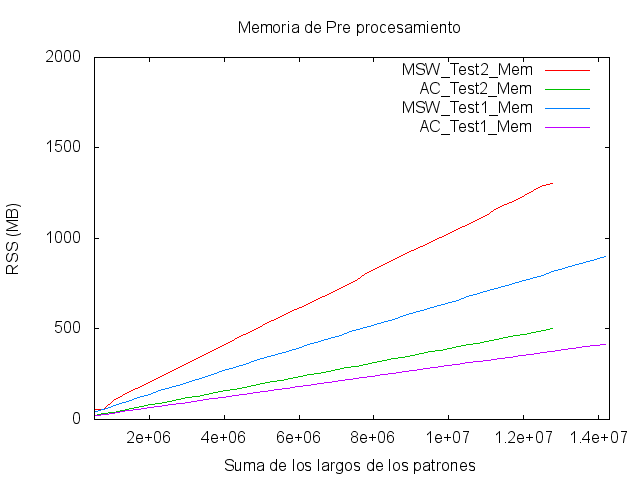
\includegraphics[scale=0.5]{Ubuntu_50PatsVsMultiPats_preprocesamiento.png}
		\rule{35em}{0.5pt}
	\caption[gráfica RSS]{Memoria residente (RSS en Ubuntu)}
	\label{fig:Memoria50PatsVsMultiPats}
\end{figure}
En ambos algoritmos, el tiempo de ejecución del pre procesamiento es lineal en la suma de los largos de los patrones. Sin embargo, en la práctica, se requiere más tiempo de ejecución por parte de MSW que por AC. \\
En ambos casos, los patrones son cargados en una estructura inicial.
La construcción de la clausura FSM a partir de la estructura inicial (GCT) requiere de varios ciclos de ejecución recursiva para llevar a cabo la transformación de la estructura, dentro de los cuales pueden realizarse modificaciones de los nodos existentes y creaciones de nuevos nodos. Por otro lado el algoritmo requiere una etapa final en la cual se realiza la propagación de las transiciones, esta operativa requiere recorrer toda la GCT. Mientras tanto, AC, luego de cargar la estructura básica en memoria no necesita insertar más nodos. Este algoritmo recorre una única vez su estructura agregando elementos al conjunto {\it “output”} y generando la función de fallos en forma iterativa.
Resulta entonces que MSW debe realizar una operativa más compleja en la fase de pre procesamiento que AC.\\
Por esta razón, es esperable, y así fue confirmado experimentalmente, que en la fase de pre procesamiento se obtengan tiempos de ejecución mayores por parte de MSW que de AC.\\
La gráfica \ref{fig:Tiempo50PatsVsMultiPats} presenta el tiempo total de la fase de pre procesamiento para diferentes pruebas. En el eje de las abscisas se presenta el largo total de caracteres procesados, mientras que en el eje Y se muestra el tiempo medido en segundos. Los gráficos AC\_Test1\_T y MSW\_Test1\_T corresponden a la medición del tiempo de pre procesamiento de la prueba 1 para los algoritmos AC y MSW respectivamente, mientras que AC\_Test2\_T y MSW\_Test2\_T presenta los gráficos para la prueba 2.\\
De esta representación observamos que los tiempos evolucionan linealmente en todos los casos, no obstante, a igual cantidad de caracteres total del archivo de patrones, MSW tarda más en procesar patrones suficientemente largos que muchos cortos. Un comportamiento inverso tiene AC, este algoritmo tarda más en procesar un conjunto considerable de patrones (con largo chico) que en realizar la misma tarea con pocos patrones de largo considerable (en relación a consideraciones de MSW).\\
Comparativamente AC es más veloz que MSW en las dos configuraciones pero cabe destacar que para la prueba 1 la diferencia máxima es del entorno de 12 segundos mientras que la diferencia máxima en la prueba 2 es más de 12 segundos\\
Pruebas similares, con otras configuraciones de cantidad de patrones fijo y rangos de largo fijo arrojaron tendencias similares al ser ejecutadas en los dos ordenadores de prueba.\\
\begin{figure}[htbp]
	\centering
		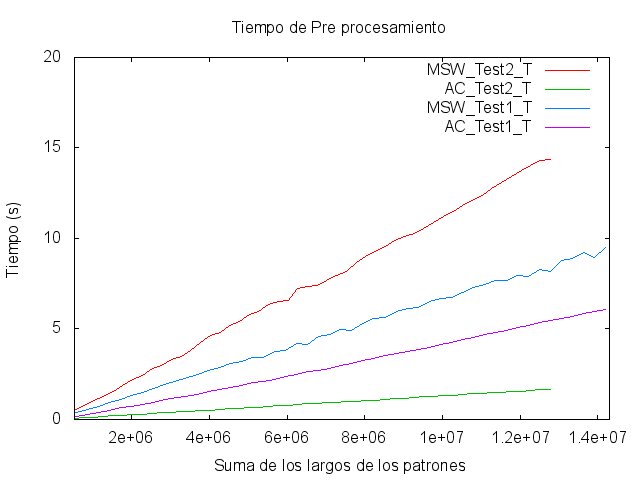
\includegraphics[scale=0.5]{Ubuntu_50PatsVsMultiPats_preprocesamiento_tiempo.png}
		\rule{35em}{0.5pt}
	\caption[gráfica tiempo de ejecución de pre procesamiento]{Tiempo de ejecución de pre procesamiento (medido en Ubuntu)}
	\label{fig:Tiempo50PatsVsMultiPats}
\end{figure}
\section{Procesamiento sobre textos}
\label{sec:procesamiento}
En la sección anterior analizamos los algoritmos en la etapa de pre procesamiento. Dicha fase genera las estructuras de datos necesarias para realizar la búsqueda del conjunto de patrones sobre el texto contenido en un archivo.\\
El archivo de texto es leído de disco a memoria secuencialmente en bloques de tamaño fijo. Cada uno de los bloques es procesado cáracter a cáracter por el programa principal en ambos algoritmos. El procedimiento por el cual se realiza la lectura de cada archivo es compartido por ambos algoritmos, de modo que los costos de cómputo y consumo de memoria  asociados a esta tarea son idénticos en ambos casos. 
Los algoritmos registran los hallazgos de correspondencia entre una secuencia de caracteres leída y los patrones que se están buscando. A partir de los datos registrados el programa puede generar un informe de la búsqueda al finalizar la recorrida sobre el texto. En nuestras pruebas, este informe consiste en la cantidad de veces que fue hallado cada uno de los patrones. En el caso de MSW, la información persistida no es suficiente, ya que, como se vió en el capítulo \ref{Chapter3}, es necesario realizar un post procesamiento para obtener los resultados finales.\\
Como se explicó en el capítulo \ref{Chapter3}, es posible liberar parte de la memoria utilizada por el algoritmo MSW luego de la fase de pre procesamiento. Sin embargo, dicha liberación no fue implementada en este proyecto. Dado que el procesamiento sobre el texto se realiza en bloques de tamaño fijo, el consumo global de memoria queda esencialmente determinada por la etapa de pre procesamiento.
Por esta razón, se considera un conjunto de pruebas que tienen como fin examinar los tiempos de ejecución de ambos algoritmos en la fase de procesamiento del texto y omitimos la evaluación del consumo de memoria en esta etapa.
Estos conjuntos son examinados contra los diferentes texto de prueba, tomando los tiempos de procesamiento del texto (recorrida y hallazgo de los múltiples patrones). 

\subsection{Efecto del conjunto de patrones sobre el tiempo de procesamiento de texto}
Al igual que en la sección \ref{sec:pre_procesamiento}, analizamos el comportamiento de los algoritmos ante variaciones en el largo y la cantidad de patrones. Se ejecutaron las cuatro pruebas especificadas en el cuadro \ref{tab:Definicion_Pruebas}, cada una de ellas sobre cuatro \emph{textos} diferentes. En estas pruebas se midió el tiempo de procesamiento de cada texto completo, omitiéndose el tiempo de pre y post procesamiento.
Comenzamos presentando las gráficas de la figura \ref{fig:Prueba1Tab}, correspondientes a la ejecución de la prueba 1 sobre los \emph{textos} de prueba. Observamos en las mismas que AC presenta una ventaja en relación a MSW hasta cierto punto, a partir del cual, MSW se mantiene por debajo de la curva de AC. 
\begin{figure}[H]
\centering
	\subfigure[Anolis]{%
	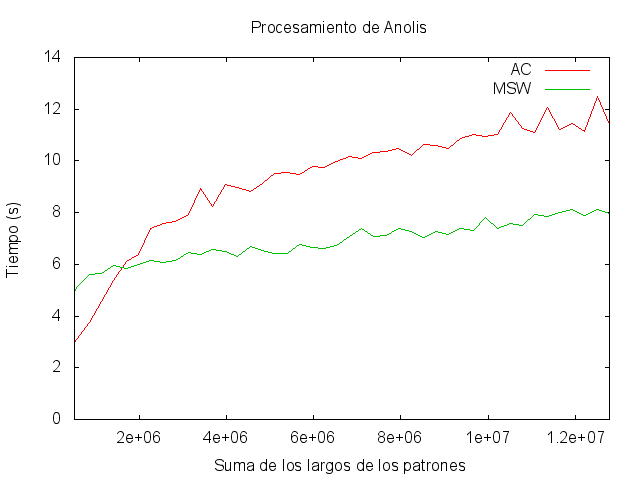
\includegraphics[scale=0.4]{Maci5_Procesamiento_Test1_Anolis.png}
	\label{fig:Prueba1Tab_a}}
\quad
	\subfigure[Canis]{%
	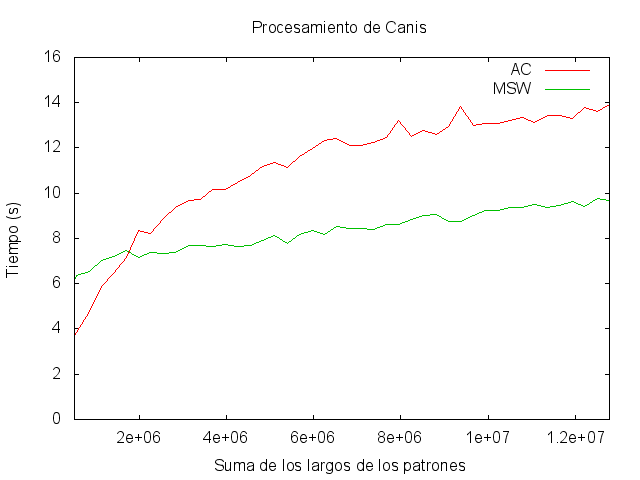
\includegraphics[scale=0.4]{Maci5_Procesamiento_Test1_Canis.png}
	\label{fig:Prueba1Tab_b}}
\quad
	\subfigure[Gallus]{%
	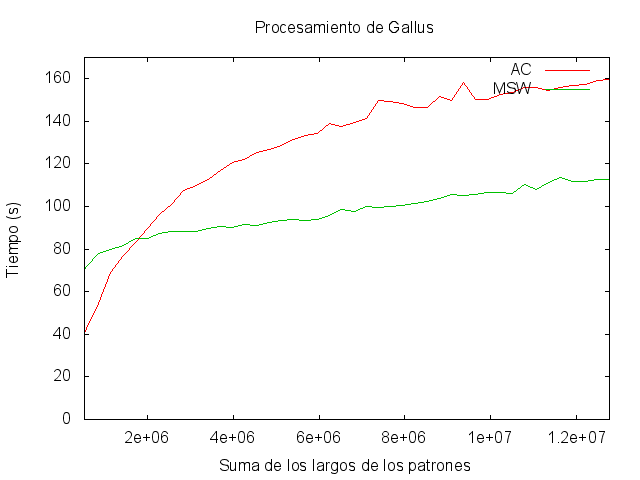
\includegraphics[scale=0.4]{Maci5_Procesamiento_Test1_Gallus.png}
	\label{fig:Prueba1Tab_c}}
\quad
	\subfigure[Homo Sapiens]{%
	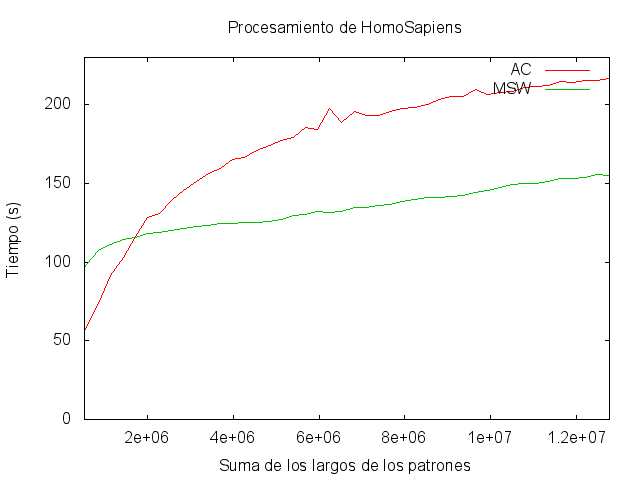
\includegraphics[scale=0.4]{Maci5_Procesamiento_Test1_HomoSapiens.png}
	\label{fig:Prueba1Tab_d}}
\caption{Tiempos de procesamiento de la prueba 1 (medido en Mac)}
\label{fig:Prueba1Tab}
\end{figure}
Cabe destacar que la prueba 1 puede contener hasta 400.000 patrones de largo corto, factor que afecta a AC, ya que aumenta la probabilidad de encontrar patrones dentro de los \emph{textos} de prueba (ver introducción del capítulo \ref{Chapter2}). Este hecho, mitiga la ventaja en consumo de memoria que tiene AC sobre MSW.
Por contra parte, al analizar las gráficas presentadas en la figura \ref{fig:Prueba2Tab}, correspondientes a la prueba 2, observamos que AC se mantiene casi constante mientras MSW es siempre creciente. 
\begin{figure}[H]
\centering
	\subfigure[Anolis]{%
	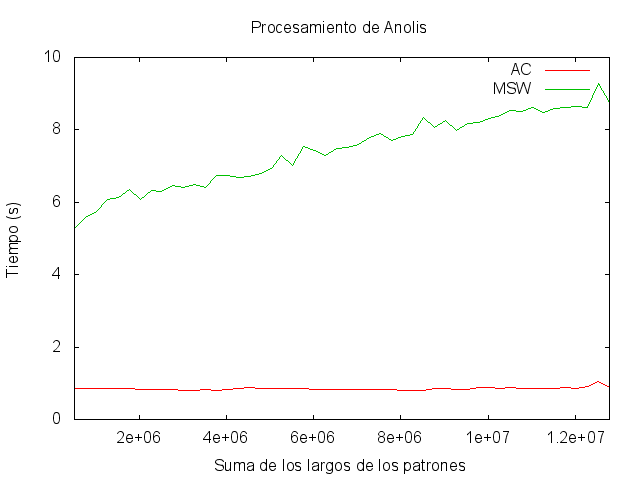
\includegraphics[scale=0.4]{Maci5_Procesamiento_10PatsCortos_Anolis.png}
	\label{fig:Prueba2Tab_a}}
\quad
	\subfigure[Canis]{%
	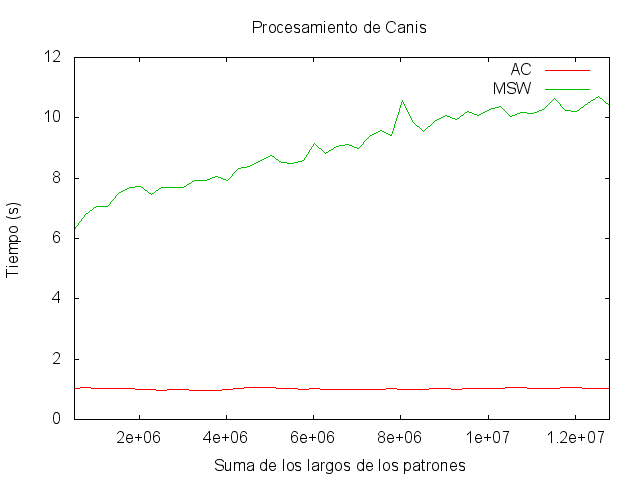
\includegraphics[scale=0.4]{Maci5_Procesamiento_10PatsCortos_Canis.png}
	\label{fig:Prueba2Tab_b}}
\quad
	\subfigure[Gallus]{%
	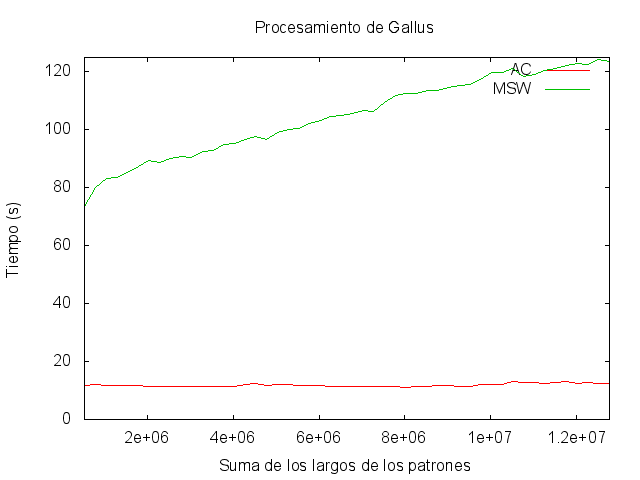
\includegraphics[scale=0.4]{Maci5_Procesamiento_10PatsCortos_Gallus.png}
	\label{fig:Prueba2Tab_c}}
\quad
	\subfigure[Homo Sapiens]{%
	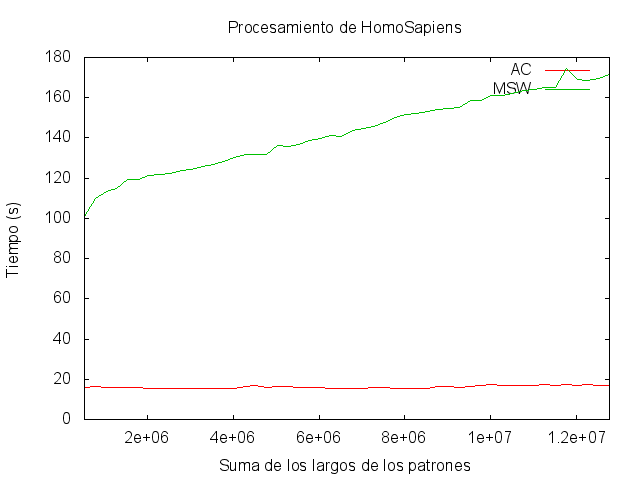
\includegraphics[scale=0.4]{Maci5_Procesamiento_10PatsCortos_HomoSapiens.png}
	\label{fig:Prueba2Tab_d}}
\caption{Tiempos de procesamiento de la prueba 2 (medido en Mac)}
\label{fig:Prueba2Tab}
\end{figure}
Los resultados de la prueba 3, presentados en la figura \ref{fig:Prueba3Tab}, se observa una clara ventaja de MSW sobre AC. La configuración usada en esta prueba es similar a la de la prueba 1, solo que el largo y la cantidad de patrones utilizada es mucho más pequeña que en la prueba 1.
\begin{figure}[H]
\centering
	\subfigure[Anolis]{%
	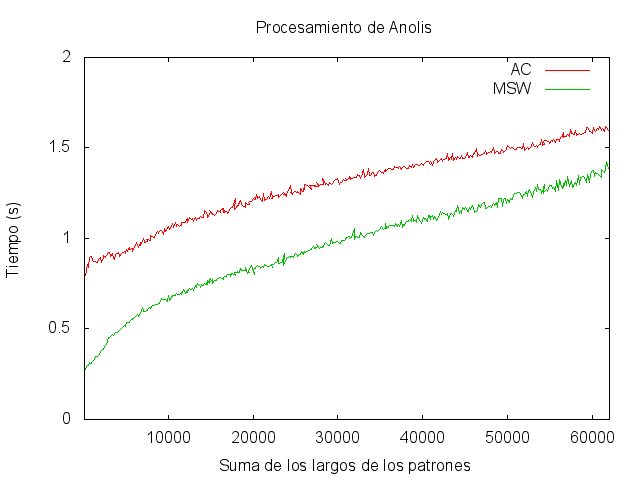
\includegraphics[scale=0.4]{Maci5_PequenosPatrones_Anolis.png}
	\label{fig:Prueba3Tab_a}}
\quad
	\subfigure[Canis]{%
	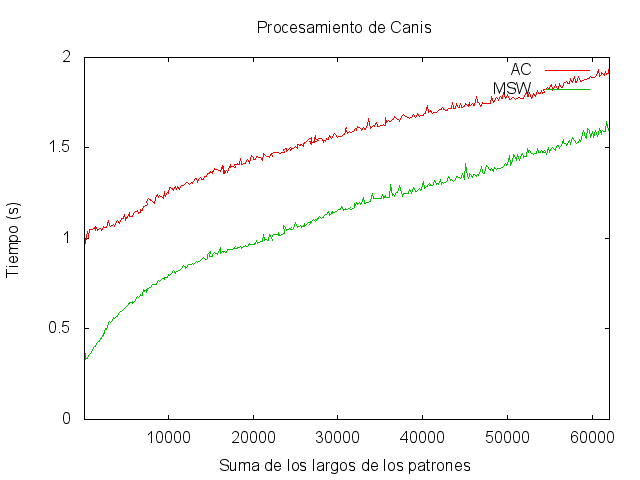
\includegraphics[scale=0.4]{Maci5_PequenosPatrones_Canis.png}
	\label{fig:Prueba3Tab_b}}
\quad
	\subfigure[Gallus]{%
	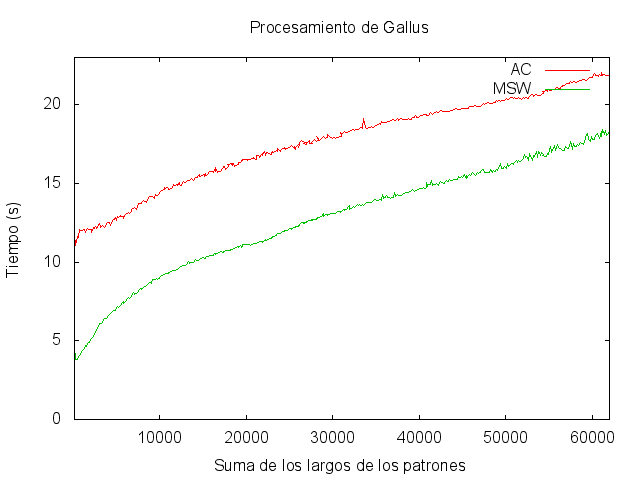
\includegraphics[scale=0.4]{Maci5_PequenosPatrones_Gallus.png}
	\label{fig:Prueba3Tab_c}}
\quad
	\subfigure[Homo Sapiens]{%
	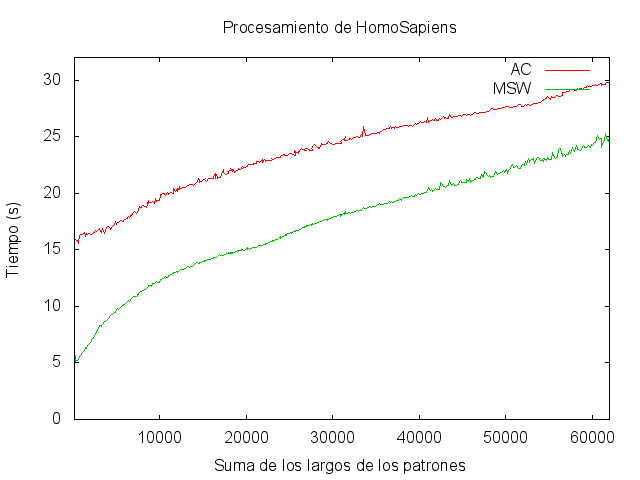
\includegraphics[scale=0.4]{Maci5_PequenosPatrones_HomoSapiens.png}
	\label{fig:Prueba3Tab_d}}
\caption{Tiempos de procesamiento de la prueba 3 (medido en Mac)}
\label{fig:Prueba3Tab}
\end{figure}
Al igual que en la prueba 2, los resultados de la prueba 4, presentados en la figura \ref{fig:Prueba4Tab}, muestran que los tiempos de procesamiento de AC tienen un comportamiento casi constante, mientras que para MSW la misma curva es siempre creciente. En el caso de la prueba 4 se tiene que, a partir de una cantidad de caracteres (suma total) de patrones, AC obtiene mejores tiempos de ejecución que MSW. En la prueba 2, por tratarse de muestras con largo total de caracteres varias unidades mayores que las usadas en la prueba 4, la curva descrita por MSW siempre se muestra por encima de la de AC.
\begin{figure}[H]
\centering
	\subfigure[Anolis]{%
	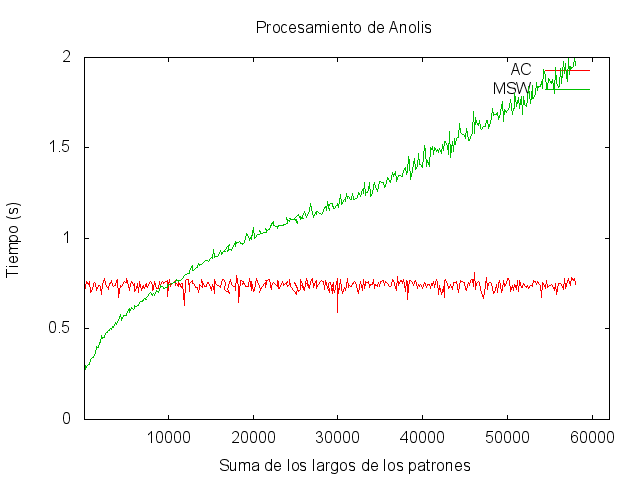
\includegraphics[scale=0.4]{Maci5_10PatsCortos_Anolis.png}
	\label{fig:Prueba4Tab_a}}
\quad
	\subfigure[Canis]{%
	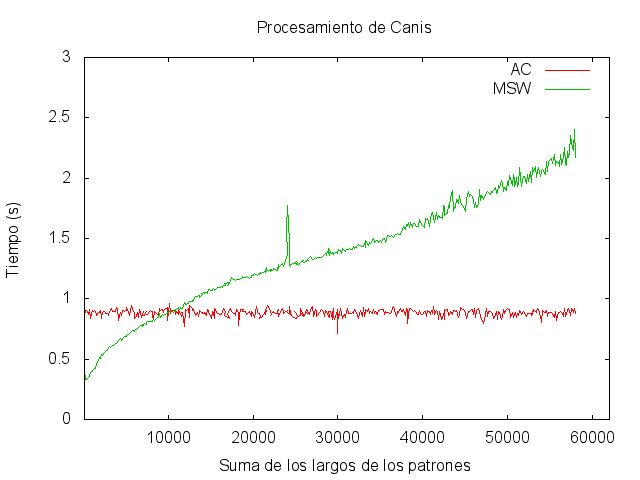
\includegraphics[scale=0.4]{Maci5_10PatsCortos_Canis.png}
	\label{fig:Prueba4Tab_b}}
\quad
	\subfigure[Gallus]{%
	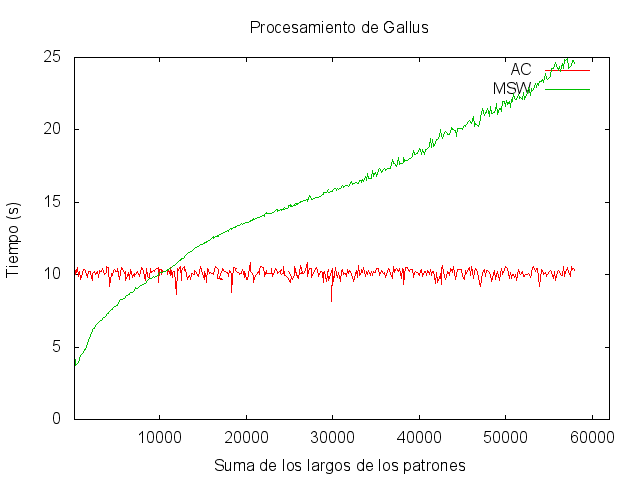
\includegraphics[scale=0.4]{Maci5_10PatsCortos_Gallus.png}
	\label{fig:Prueba4Tab_c}}
\quad
	\subfigure[Homo Sapiens]{%
	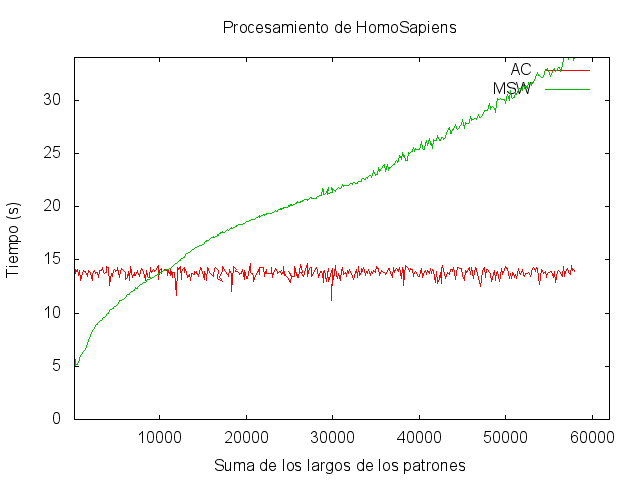
\includegraphics[scale=0.4]{Maci5_10PatsCortos_HomoSapiens.png}
	\label{fig:Prueba4Tab_d}}
\caption{Tiempos de procesamiento de la prueba 4 (medido en Mac)}
\label{fig:Prueba4Tab}
\end{figure}
A pesar de tener una cantidad total de caracteres de patrones similares a la prueba 4, la prueba 3 arroja diferentes resultados (esto también sucede si comparamos las pruebas 1 y 2). Esta comparación muestra que al variar el largo y la cantidad de patrones (conservando la suma de los caracteres) se obtienen diferencias entre estos algoritmos.
A pesar de que la segunda etapa de MSW es más sencilla que la de AC, lo cual haría esperar que fuera más eficiente es posible encontrar configuraciones en las cuales el tiempo de ejecución de la segunda etapa de MSW es mayor que la de  AC.
La figura \ref{fig:exp2_2Tab} resume estas observaciones.
\begin{figure}[H]

\centering
	\subfigure[Prueba 1]{%
	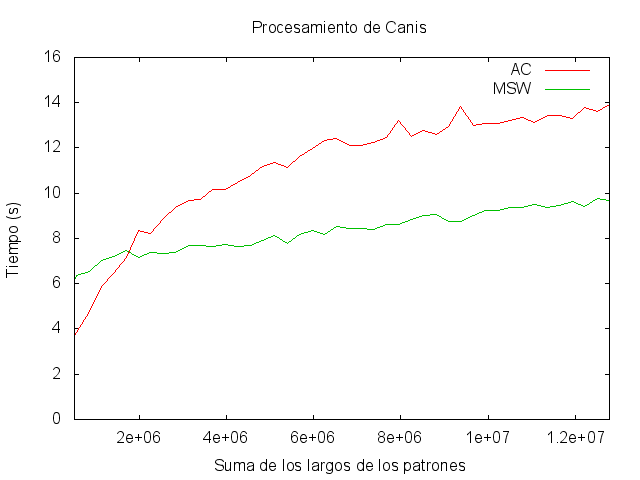
\includegraphics[scale=0.4]{Maci5_Procesamiento_Test1_Canis.png}
	\label{fig:exp2_2Tab_a}}
\quad
	\subfigure[Prueba 2]{%
	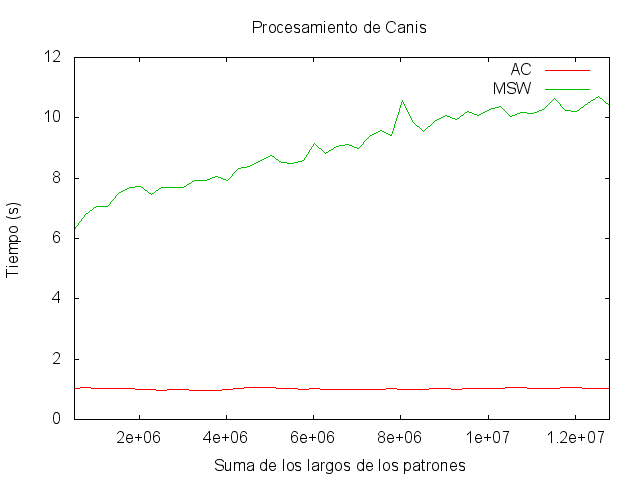
\includegraphics[scale=0.4]{Maci5_Procesamiento_10PatsCortos_Canis.png}
	\label{fig:exp2_2Tab_b}}
\quad
	\subfigure[Prueba 3]{%
	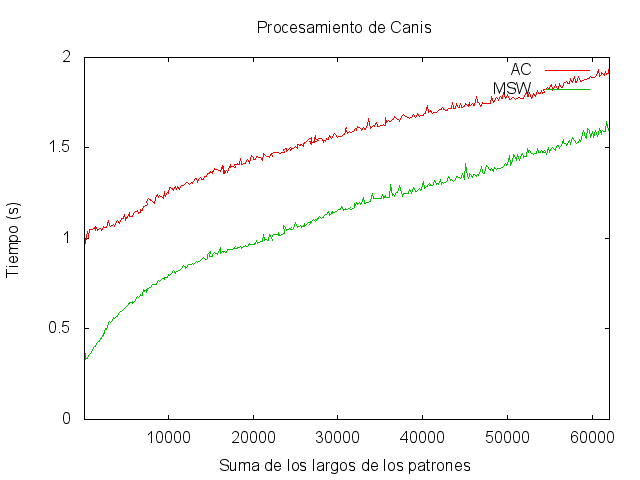
\includegraphics[scale=0.4]{Maci5_PequenosPatrones_Canis.png}
	\label{fig:exp2_2Tab_c}}
\quad
	\subfigure[Prueba 4]{%
	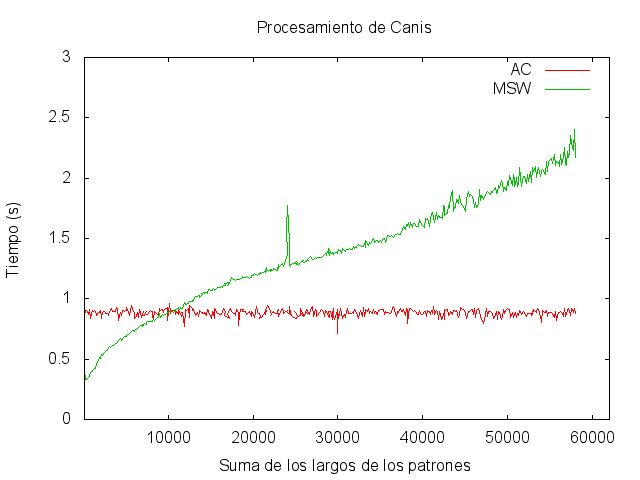
\includegraphics[scale=0.4]{Maci5_10PatsCortos_Canis.png}
	\label{fig:exp2_2Tab_d}}
\caption{Comparación de tiempos entre las pruebas 1, 2, 3 y 4 (medido en Mac)}
\label{fig:exp2_2Tab}
\end{figure}
\subsection{Efecto de los fallos de memoria caché en el rendimiento de los algoritmos}
\label{subsec:falloscache}
Con el fin de comprender estos resultados, se analiza la situación de la memoria caché en la ejecución de ambos algoritmos. Se utilizó el programa $\href{http://valgrind.org/}{Valgrid}$ \footnote{Sitio web de Valgrid - http://valgrind.org/} para simular algunas ejecuciones sobre los juegos de pruebas tres y cuatro. Las simulaciones fueron realizadas en Mac y Ubuntu, los datos presentados en este documento corresponden a las ejecuciones sobre Mac; no obstante, en Ubuntu se obtuvieron similares resultados.\\
Las medidas que se consideran en el análisis son:
\begin{itemize}
\item  {\it Ir} : Número de instrucciones ejecutadas.
\item  {\it Dr} : Número de accesos a caché.
\item  {\it D1 misses} : Número de fallos de lectura + fallos de escritura en el nivel 1 del caché.
\item  {\it LLd misses} : Número de fallos de lectura + fallos de escritura en el último nivel del caché.
\item  {\it D1MR} : La tasa de fallos de caché de nivel 1, la cual se define en \cite{bruce07} como $\frac{D1 misses}{Dr}$
\end{itemize}

\begin{table}[H]
\begin{center}
\scalebox{0.5} {
\begin{tabular}{lllllllllll}
\hline
  Total de caracteres\\ de patrones & \multicolumn{4}{c}{AC} & \multicolumn{4}{c}{MSW}\\

 & Ir & Dr & D1 misses & LLd misses  & D1MR  
 & Ir & Dr & D1 misses & LLd misses & D1MR  \\
  \midrule
152&2,234,416,638&1,100,639,130&1,468,835&1,436,691&	0.1	&1,650,365,936&914,344,784&1,505,777&1,437,163&	0.1\\
7711&2,311,573,313&1,145,950,533&73,772,855&1,451,051&	6.4	&1,659,976,386&918,092,533&109,984,409&1,472,333&	11.9\\
15464&2,312,674,348&1,145,689,265&118,963,702&1,467,023&	10.3	&1,670,302,224&921,759,044&122,377,389&1,516,200&	13.2\\
23168&2,313,449,124&1,145,256,163&140,564,456&1,484,593&	12.2	&1,681,348,889&925,424,216&126,393,101&1,577,561&	13.6\\
31075&2,321,743,241&1,149,328,728&153,739,533&1,505,375&	13.3	&1,689,027,898&928,660,247&128,533,849&1,671,861&	13.8\\
38774&2,326,427,056&1,151,276,154&160,771,680&1,528,210&	13.9	&1,699,780,189&932,164,070&130,134,560&1,876,071&	13.9\\
46293&2,330,888,470&1,153,133,794&166,657,548&1,551,410&	14.4	&1,706,350,880&934,938,423&130,801,571&2,222,245&	13.9\\
54244&2,335,825,040&1,155,214,790&171,046,365&1,583,281&	14.8	&1,717,504,016&938,584,651&132,001,853&2,918,619&	14\\
61981&2,343,747,921&1,159,143,991&175,323,573&1,617,820&	15.1	&1,724,797,823&941,448,518&132,382,025&4,025,800&	14\\
  \bottomrule
\end{tabular} }
\captionof{table}{Datos de caché de la prueba 3 sobre el texto Canis} \label{tab:Prueba1Cache} 
\end{center}
\end{table}

\begin{table}[H]
\begin{center}
\scalebox{0.5} {
\begin{tabular}{lllllllllll}
\hline
  Total de caracteres\\ de patrones & \multicolumn{4}{c}{AC} & \multicolumn{4}{c}{MSW}\\

 & Ir & Dr & D1 misses & LLd misses  & D1MR  
 & Ir & Dr & D1 misses & LLd misses & D1MR  \\
  \midrule
152&2,234,401,677&1,100,635,524&1,468,822&1,436,679&	0.1	&1,650,350,975&914,341,178&1,505,738&1,437,141&	0.1\\
7221&2,218,051,314&1,089,754,707&1,485,822&1,443,909&	0.1	&1,667,205,338&920,557,984&114,142,061&1,472,818&	12.3\\
14474&2,326,341,972&1,153,639,885&1,504,891&1,451,340&	0.1	&1,684,805,417&926,961,265&124,963,029&1,512,145&	13.4\\
21678&2,346,109,041&1,164,412,795&1,515,997&1,458,684&	0.1	&1,702,442,826&933,386,701&128,446,457&1,615,262&	13.7\\
29085&2,337,255,660&1,157,984,784&1,532,988&1,466,148&	0.1	&1,721,099,238&940,044,561&131,244,588&1,866,211&	13.9\\
36284&2,343,421,387&1,160,598,094&1,549,925&1,473,574&	0.1	&1,739,546,344&946,515,236&132,295,339&2,637,328&	13.9\\
43303&2,343,395,748&1,159,522,319&1,562,490&1,480,773&	0.1	&1,757,495,713&952,801,842&133,099,606&4,500,478&	13.9\\
50754&2,282,819,598&1,122,060,519&1,578,185&1,495,522&	0.1	&1,776,786,022&959,530,443&134,493,371&7,875,837&	14.0\\
57991&2,386,121,854&1,182,942,024&1,590,988&1,523,510&	0.1	&1,795,440,485&966,083,880&135,150,380&12,046,266&	13.9\\
  \bottomrule
\end{tabular} }
\captionof{table}{Datos de caché de la prueba 4 sobre el texto Canis} \label{tab:Prueba2Cache} 
\end{center}
\end{table}

Como se muestra en los cuadros \ref{tab:Prueba1Cache} y \ref{tab:Prueba2Cache}, la implementación de la segunda etapa del algoritmo MSW ejecuta siempre menos instrucciones que la de AC. Se puede apreciar que en la situación del cuadro \ref{tab:Prueba1Cache}, ambos algoritmos presentan una tasa similar de fallos de caché de nivel uno, que es creciente con la suma de los largos de los patrones. Esto es consistente con la figura \ref{fig:exp2_2Tab_c}, en la cual los tiempos de ejecución son crecientes tanto para MSW como para AC, estando la curva de MSW siempre por debajo de la de AC.\\
En el cuadro \ref{tab:Prueba2Cache}, en cambio observamos que la tasa de fallos de caché de nivel uno en MSW tiene un comportamiento similar al del cuadro \ref{tab:Prueba1Cache}, pero la tasa de fallos de caché de nivel uno de AC se mantiene constante y nunca supera a la de MSW. Esto es nuevamente consistente con la figura \ref{fig:exp2_2Tab_d}, donde el tiempo de ejecución de AC se mantiene aproximadamente constante. Para instancias suficientemente grandes, el mejor aprovechamiento de la memoria caché termina inclinando la balanza a favor de AC.\\
Otra medida recogida de las pruebas es la cantidad de fallos de memoria caché del último nivel, para MSW, la misma presenta un crecimiento abrupto en las últimas filas de los cuadros \ref{tab:Prueba1Cache} y \ref{tab:Prueba2Cache}, siendo más notorio en el cuadro \ref{tab:Prueba2Cache}. Por su lado, la cantidad de fallos de memoria caché del último nivel de AC no varía de forma considerable en ningún caso.\\
De lo analizado anteriormente y resultados obtenidos en otros experimentos que no se presentan en este documento por arrojar resultados similares a los ya presentados, se puede concluir que los fallos de memoria caché, así como los de página (en memoria principal) redundan negativamente en el rendimiento de los algoritmos presentados. En condiciones en las cuales estos fallos afectan a ambos algoritmos de forma equitativa MSW obtendrá mejores tiempos que AC, sin embargo, para juegos de patrones configurados de forma tal que la estructura de AC obtenga baja tasa de fallos de caché este último algoritmo superará a MSW. En particular, tomando juegos de pruebas con patrones suficientemente largos MSW consumirá una cantidad de memoria que puede llevar a que el sistema produzca más fallos de caché y de página (enlenteciendo la ejecución) comparado con AC.
\subsubsection{Efecto del largo del texto sobre el tiempo de procesamiento de texto}
Una observación pertinente es que a lo largo del procesamiento de los texto, el tiempo de ejecución medido en cada bloque de lectura presenta una variación muy pequeño. Esta afirmación se observa en las gráficas presentadas en la figura \ref{fig:bloques_procesados}, donde el eje Y representa el tiempo de ejecución por bloque del procesamiento sobre el texto {\it HomoSapiens} y el eje X representa la suma de los largos de los patrones. Se ejecutaron once juegos de patrones correspondientes a la prueba 3 (figura \ref{fig:bloque_3}) y prueba 4 (figura \ref{fig:bloque_4}).\\
En cada ejecución se midió el tiempo del procesamiento de cada uno de los 340 bloques, cada uno de aproximadamente 4MB. En estas gráficas se muestra el promedio de los tiempos obtenidos en cada experimento. También se presenta, en cada punto, una barra que representa la desviación estándar en los datos medidos.
\begin{figure}[H]
\centering
	\subfigure[Prueba 3]{%
	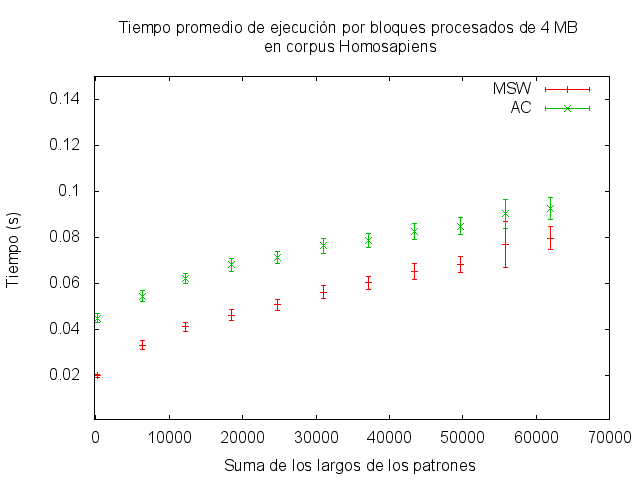
\includegraphics[scale=0.4]{Mac_DesviacionEstandar_Test3.png}
	\label{fig:bloque_3}}
\quad
	\subfigure[Prueba 4]{%
	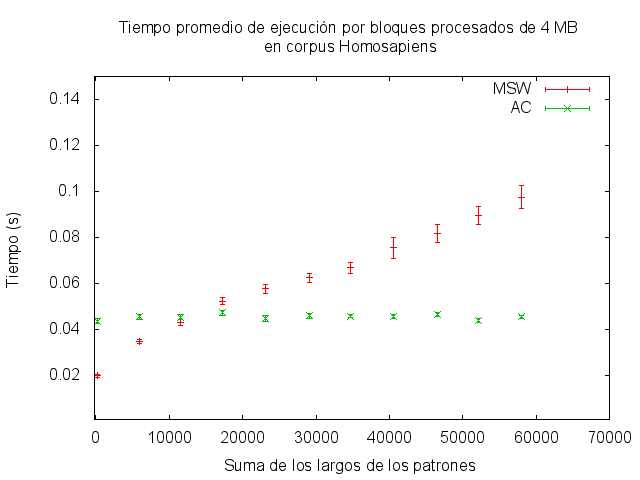
\includegraphics[scale=0.4]{Mac_DesviacionEstandar_Test4.png}
	\label{fig:bloque_4}}
\caption{Tiempo promedio de procesamiento por bloques de lectura (medido en Mac)}
\label{fig:bloques_procesados}
\end{figure}
\section{Tiempo total de ejecución}
En esta sección se presentan los resultados de los tiempos totales de ejecución en las diversas pruebas ejecutadas. 
Para este análisis definimos tiempo total como $t_{f}$ = $t_{pre}$ + $t_{pro}$ + $t_{pos}$, siendo $t_{pre}$ el tiempo de ejecución del pre procesamiento (creación de la estructuras) analizado en la sección \ref{sec:pre_procesamiento}, $t_{pro}$ el tiempo de ejecución del procesamiento del texto (abordado en la sección \ref{sec:procesamiento}) y  $t_{pos}$ el tiempo de post procesamiento. Para el tiempo de post procesamiento no se considera el tiempo de impresión de datos, por lo que, para el algoritmo AC este tiempo es nulo. El algoritmo MSW presenta una fase de post procesamiento, sin embargo pudo comprobarse que la misma es despreciable.\\ 
El tiempo de ejecución total en las pruebas 1 y 2 presentan $t_{pre}$ apreciable. En el caso de las prueba 1, existe un pequeño intervalo en el cual AC presenta ventaja respecto a MSW, luego del cual MSW siempre obtiene mejores tiempos, tanto de procesamiento como totales. Como se ha mencionado anteriormente, el tiempo de pre procesamiento siempre ubica al algoritmo AC con clara ventaja respecto a MSW, sin embargo, en algunas circunstancias, esta ventaja inicial no termina repercutiendo a su favor al recorrer \emph{textos} suficientemente largos. \\
En el cuadro \ref{tab:Total1} se presentan algunos tiempos totales y de procesamiento de la prueba 1. 

\begin{table}[H]
\begin{center}
\scalebox{0.7} {
\begin{tabular}{lllll}
\hline
  Total de caracteres\\ de patrones & \multicolumn{2}{c}{AC} & \multicolumn{2}{c}{MSW}\\

 & $t_{pro}(s)$ & $t_{f}(s)$
 & $t_{pro}(s)$ & $t_{f}(s)$ \\
  \midrule
    284134&42.02&42.11&81.15&81.28\\
    852382&73.64&73.85&107.13&107.51\\
    7952292&197.64&200.03&138.53&142.14\\
    9938725&206.53&209.57&145.75&151.09\\
    14202416&219.86&224.26&159.42&166.09\\
  \bottomrule
\end{tabular}
}
\captionof{table}{Algunos valores de tiempos totales de la prueba 1 sobre el texto HomoSapiens}
\label{tab:Total1} 
\end{center}
\end{table}

El cuadro \ref{tab:Total2} corresponde a algúnos valores tomados en la prueba 2. En dicho cuadro, se muestra en números, la clara ventaja que presenta AC sobre MSW en dicha configuración de prueba.
\begin{table}[H]
\begin{center}
\scalebox{0.7} {
\begin{tabular}{lllll}
\hline
  Total de caracteres\\ de patrones & \multicolumn{2}{c}{AC} & \multicolumn{2}{c}{MSW}\\

 & $t_{pro}(s)$ & $t_{f}(s)$
 & $t_{pro}(s)$ & $t_{f}(s)$ \\
  \midrule
    524912&16.14&16.30&101.01&101.33\\
    2774182&15.49&16.00&123.93&125.85\\
    5274746&16.39&17.35&135.88&139.60\\
    7776769&15.44&16.85&149.97&155.79\\
    10272380&16.76&18.59&160.86&168.80\\
	12777202&16.97&19.26&171.76&181.45\\
  \bottomrule
\end{tabular}
}
\captionof{table}{Algunos valores de tiempos totales de la prueba 2 sobre el texto HomoSapiens}
 \label{tab:Total2}
\end{center}
\end{table}
  
En el cuadro \ref{tab:Total3} se presentan algunos tiempos totales de la prueba 3, como puede apreciarse, MSW mantiene su ventaja respecto de AC. Se observa en ese cuadro que la diferencia entre el tiempo de procesamiento y el tiempo total de ejecución, es decir, $t_{pre}$, es casi despreciable; esto se debe a que la suma de los largos de los patrones que se usaron en la prueba son relativamente pequeños en comparación a los de las muestras utilizadas en las pruebas 1 y 2. De este razonamiento se desprende, y así fue comprobado en pruebas, que los tiempos totales de ejecución de la prueba 4 son equivalentes a los del procesamiento mostrados en la sección \ref{sec:procesamiento}. Por dicho motivo se omitió la presentación de la tabla de tiempos totales de la prueba 4.  
\begin{table}[H]
\begin{center}
 
\scalebox{0.7} {
\begin{tabular}{lllll}
\hline
  Total de caracteres\\ de patrones & \multicolumn{2}{c}{AC} & \multicolumn{2}{c}{MSW}\\

 & $t_{pro}(s)$ & $t_{f}(s)$
 & $t_{pro}(s)$ & $t_{f}(s)$ \\
  \midrule
    152&15.957630&15.957846&6.241849&6.242040\\
    3138&16.600447&16.601562&8.289137&8.290025\\
    4721&17.226274&17.227594&9.458761&9.460374\\
    15464&21.018896&21.021923&14.07945&14.084688\\
    23168&22.973389&22.977644&15.792082&15.797569\\
    38774&25.932629&25.939657&19.634354&19.644133\\
    54244&28.208693&28.217854&22.898829&22.911264\\
    61981&29.803581&29.813734&24.967764&24.982885\\
  \bottomrule
\end{tabular}
}
\captionof{table}{Algunos valores de tiempos totales de la prueba 3 sobre el texto HomoSapiens}
 \label{tab:Total3}
\end{center}
\end{table}
\section{Conclusiones}
En este capítulo se presentó un análisis cuantitativo que muestra las fortalezas y debilidades de los algoritmos en diferentes configuraciones, comparando los tiempos de ejecución obtenidos con las mediciones de consumo de memoria principal y accesos a memoria caché. Se expusieron argumentos que justifican las mediciones obtenidas, presentando conclusiones del rendimiento de los algoritmos que fueron comparados.\\
De las pruebas experimentales surgió que existen diversas configuraciones de datos de entrada que impactan sobre el comportamiento de los algoritmos, de forma tal que en algunos casos MSW presenta mejores tiempos de ejecución (totales y de procesamiento) que AC y vice versa. El algoritmo MSW presenta mejores tiempos cuando el conjunto de patrones a ser buscado es suficientemente grande y el largo de cada patrón es relativamente pequeño. En los casos en que se tengan patrones suficientemente extensos AC presentará mejores tiempos que MSW.\\
También se observó que en todas las configuraciones AC tiene un tiempo de pre procesamiento menor que MSW, pero la diferencia entre estos se puede reducir en la segunda etapa en los casos en que la cantidad de memoria requerida por MSW no afecta negativamente el aprovechamiento de la jerarquía de memoria en mayor medida que AC.
Como trabajo futuro se plantea, dado el análisis de este capítulo, realizar mejoras en las estructuras de datos del algoritmo MSW que permitan reducir los fallos de caché.\\

%Dentro del entregable se encuentran los directorios de experimentación, los cuales contienen los scripts de ejecución de %las pruebas presentadas en este capítulo y otras que no fueron incluidas. También se encuentran los resultados obtenidos %en las ejecuciones en las distintas computadoras.

%----------------------------------------------------------------------------------------
%	THESIS CONTENT - APPENDICES
%----------------------------------------------------------------------------------------

\addtocontents{toc}{\vspace{2em}} % Add a gap in the Contents, for aesthetics

\appendix % Cue to tell LaTeX that the following 'chapters' are Appendices

% Include the appendices of the thesis as separate files from the Appendices folder
% Uncomment the lines as you write the Appendices

% Appendix A

\chapter{Programa principal - PDG} % Main appendix title

\label{AppendixA} % For referencing this appendix elsewhere, use \ref{AppendixA}
\lhead{Appendix A. \emph{Programa principal - PDG}} % This is for the header on each page - perhaps a shortened title


\begin{center}

\begin{table}
\captionof{table}{Argumentos del programa principal} \label{tab:PDGArgs} 
\begin{tabular}{l p{10cm}}

\hline\hline
Argumento & Descripción\\
\hline
-m & Modo de ejecución (algoritmo seleccionado). 1 – Aho Corasick 2 – FSM\\
-h & Imprime los argumentos aceptados por el programa\\
-q & Cantidad de patrones a ser tenidos en cuenta\\
-c & Ruta absoluta en la cual se encuentra el archivo con el texto\\
-p & Ruta en la cual se encuentra el archivo con el conjunto de patrones a ser buscados\\
-s & Tamaño del bloque de lectura del texto (tamaño de páginas). Por defecto se utiliza un blque de 1024 páginas.\\
--printMemory & Imprime los valores RSS y VSZ del proceso (solo para sistemas operativos con procfs).\\
--printPreTime & Imprime el tiempo en segundos que tarda en ejecutarse la creación de la estructura del algoritmo que se está ejecutando\\
--readTime & Imprime el tiempo en segundos que tarda en ejecutarse la lectura completa del texto
\\
--readBlockTime & Imprime el tiempo en segundos que tarda en ejecutarse un bloque de lectura del texto\\
--postTime & Imprime el tiempo en segundos que tarda en ejecutarse el post procesamiento del algoritmo (aplicable solo para MSW).\\
--totalTime & Imprime el tiempo en segundos que tarda en ejecutar completamente el algoritmo.\\
--finds & Imprime la cantidad de veces que se encontró cada uno de los patrones. \\
--printComments & Imprime comentarios a la salida con el prefijo $\#$.\\
\hline
\end{tabular}
\label{table:PDG}
\end{table}
\end{center}
% Appendix A

\chapter{Aspectos generales de la implementación} % Main appendix title

\label{AppendixB} % For referencing this appendix elsewhere, use \ref{AppendixB}

\lhead{Appendix B. \emph{Aspectos generales de la implementación}} % This is for the header on each page - perhaps a shortened title

Este apéndice tiene como cometido explicar aspectos generales de la implementación, los cuales aplican para el algoritmo AC y MSW.\\
El programa está compuesto por módulos escritos en C++ y C, los cuales son compilados utilizando GCC versión 4.2. Dentro del entregable se adjunta en el directorio "Fuentes"  un archivo {\it Makefile} que permite compilar la solución entregada en este proyecto.\\
Los módulos del empaquetado final implementan la lógica necesaria para ejecutar los algoritmos AC y MSW.\\
Todo el código desarrollado en este proyecto fue realizado por el autor del mismo salvo que se indique lo contrario.
A continuación se describe brevemente cada uno de los módulos implementados.
\begin{itemize}
\item MSWGraph - Implementa la lógica necesaria para crear la estructura del algoritmo MSW, provee métodos para actualizar la estructura de datos al procesar el texto y obtener la cantidad de ocurrencias de un patrón específico.
\item MSWNode - Especifica la estructura de cada nodo de MSW. 
\item AhoCorasickNode - Especifica la estructura de cada nodo de AC. 
\item AhoCorasickGraph - Implementa la lógica necesaria para crear la estructura de datos del algoritmo AC, provee un método para actualizar la misma a medida que se recorre el texto y almacena la cantidad de ocurrencias de cada patrón.
\item Queue - Implementa la cola utilizada en la construcción de la función {\it failure} de AC.
\item QueueNode - Implementa un nodo de {\it Queue}.
\item Memory - Implementa un conjunto de funciones usadas para obtener medidas del consumo de memoria al ejecutar los diversos algoritmos. Los macro allí implementados y los métodos {\it getPeakRSS} y  {\it getCurrentRSS} fueron obtenidos de \href{http://goo.gl/4uZJKP}{Nadeau}.
\item Main - Es el módulo principal, en el se concentra toda la lógica necesaria para leer archivos, interpretar los argumentos ingresados por el usuario y presentar los resultados finales.
\end{itemize}
Además de los módulos indicados en los puntos anteriores se creó un archivo de constantes ({\bf Const.h}), en el mismo se define un vector con todos los símbolos del alfabeto ({\bf alphabet}), el largo del mismo ({\bf ALPHABET\_SIZE}) y un arreglo, al cual nombramos \emph{ordchar}, que es utilizado para obtener en O(1) el índice que tiene asignado cada símbolo del alfabeto (representado en ASCII) en {\bf alphabet}. En este archivo de constantes se encuentra comentada la definición del macro {\bf KDEBUG}, al descomentar dicha línea se compila un conjunto de funciones útiles para realizar {\it debug}.\\
Por motivos de rendimiento todos los atributos fueron declarados como públicos, a su vez, se implementaron en los archivos .h algunos métodos simples que son invocados de forma frecuente.
\section{Lectura de archivos}
El módulo principal {\it Main} realiza la lectura del archivo de patrones y del texto. Estos archivos difieren entre sí en que en el primero cada patrón está separado entre sí por un salto de línea, mientras que al leer los textos solo se admiten caracteres pertenecientes al alfabeto previamente establecido.\\
Todas las lecturas son realizadas desde el comienzo del archivo hasta el final del mismo (lectura de izquierda a derecha). Para el caso de la lectura del juego de patrones se utiliza la función {\it getline} mientras que la lectura del texto se realiza de a bloque de caracteres de tamaño máximo configurable. El valor por defecto del tamaño del bloque de lectura es una página de memoria del sistema operativo sobre el cual se ejecuta.\\

% Appendix B

\chapter{Testing} % Main appendix title

\label{AppendixC} % For referencing this appendix elsewhere, use \ref{AppendixC}

\lhead{Apéndice B. \emph{Testing}} % This is for the header on each page - perhaps a shortened title

Se crearon doce juegos de patrones con diferentes características y doce textos los cuales son usados para probar la correctitud de los resultados finales arrojados por los algoritmos elaborados en esta tesis.\\
En las pruebas presentadas se contempla una serie de configuraciones particulares de patrones, como por ejemplo patrones que son prefijos de otros, patrones capicúa (es decir patrones que se leen igual de izquierda a derecha que de derecha a izquierda), existencia de patrones repetidos en un mismo juego y ausencia total de patrones (juego de patrones vacío). También se incluyeron en las pruebas juegos de patrones con hasta 400.000 patrones.\\ 
Los textos fueron seleccionados para probar diversos casos, entre ellos, la posibilidad que ningún patrón se encuentre, o, que por lo contrario, se encuentren todos los patrones en el textos.\\ Se comprobó, en forma manual, la correctitud de los algoritmos sobre los primeros 5 juegos de patrones contra un conjunto reducido de los textos utilizados en las pruebas.\\ Para la realización de pruebas automatizadas se creo un script {\it runAppTest.sh} el cual ejecuta todos los juegos de patrones contra todos los textos y compara la salida de los dos algoritmos. En caso de ocurrir alguna diferencia entre ambas salidas se despliega un mensaje indicando el fallo y se guarda los archivos de salida de ambos algoritmos. De esta forma se ejecuta un total de 144 pruebas automáticas de comparación entre ambos algoritmos. En la fase de desarrollo fue utilizado un conjunto de funciones para verificar la estrucutra creada por MSW. Algunas de dichas funciones permiten imprimir en pantalla la estructura de datos, comprobar la correcta inserción de patrones en fases tempranas de los algoritmos y que las estructuras finalmente generadas sean consistentes (por ejemplo dado un nodo se verifica que sus hijos tengan asignado correctamente el nodo padre). Para utilizar las funciones de pruebas se debe definir el macro {\it KDEBUG}.\\ Los juegos de pruebas mencionados en este apéndice pueden ser encontrados bajo el directorio {\it"Testing"} del entregable.

\addtocontents{toc}{\vspace{2em}} % Add a gap in the Contents, for aesthetics

\backmatter

%----------------------------------------------------------------------------------------
%	BIBLIOGRAPHY
%----------------------------------------------------------------------------------------

\bibliographystyle{plain}
\bibliography{Referencias}
\end{document}
